\chapter{Строение атома}

\section{\# Как всё начиналось}

\begin{wrapfigure}{l}{0.35\textwidth}
    \centering
    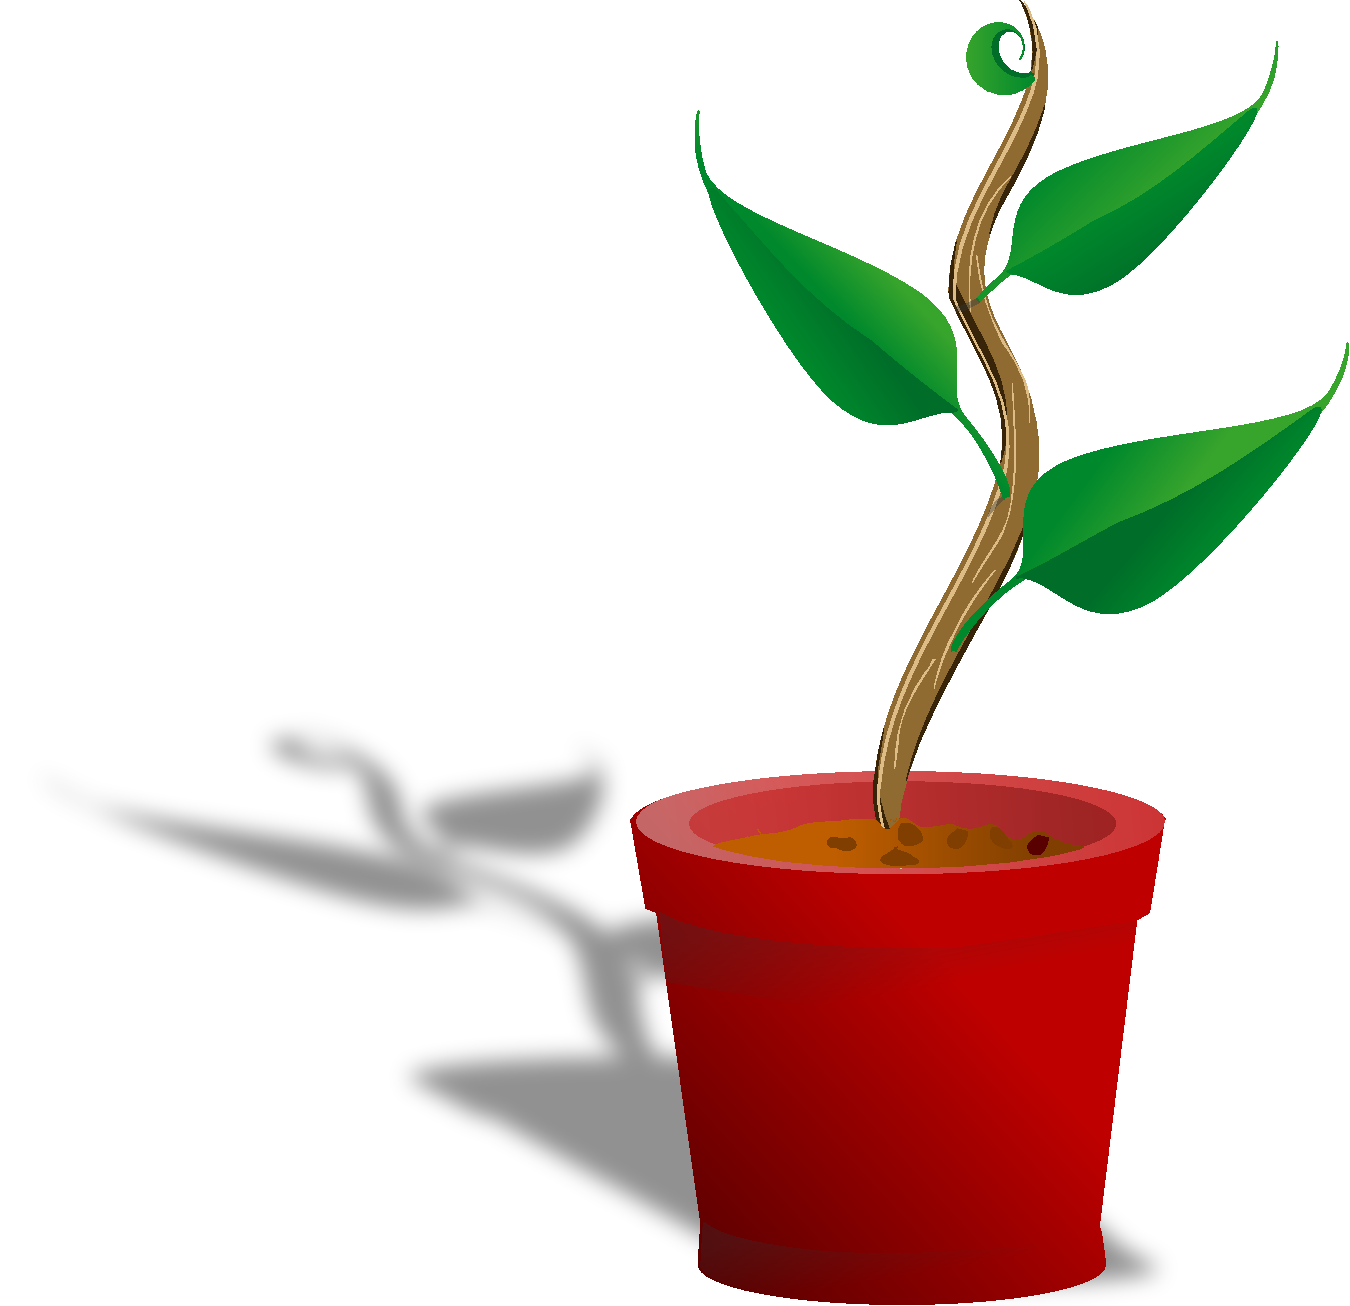
\includegraphics[width=4cm]{figs/how_it_started/flower.pdf}
\end{wrapfigure}

\hspace*{\parindent}Прежде чем мы сможем приступить непосредственно к изучению самого предмета химии, мы должны посвятить некоторое время изучению базовых знаний, без которых понять многие вещи впоследствии будет трудновато.

Как мы уже упоминали, без физических представлений об атоме невозможно понять химические превращения. Мы начнём с изучения того, как устроен атом.

На самом деле физика и химия~--- сейчас это уже скорее условности. Границы между науками вообще постепенно размываются, специалисты в естественных науках обязаны знать и то, и другое, и третье.

Вот вам три принципа, по которым хороший химик отличается от обычного, вам нужно запомнить их:

\begin{enumerate}[label=\arabic*)]
    \item \textbf{Системное мышление}\label{term:systematic_thinking}\index{системное мышление}.
    \item Умение ответить на вопрос <<\emph{Что является движущей силой?}>> для каждого явления.
    \item Не только теоретические знания, но и обладание навыками практической работы.
\end{enumerate}

Обратите внимание на первый принцип. Мыслить системно~--- это означает не запоминать отдельные разрозненные факты, а понимать базовые законы и причины, по которым происходят различные вещи, и каждый случай рассматривать с точки зрения общих закономерностей.

Самый главный принцип, который химик должен уметь объяснить,~--- \emph{почему протекает тот или иной процесс}. Попробуйте смотреть на вещи с этой точки зрения, и сами увидите, как изменится качество ваших знаний.

В этом разделе мы немного погрузимся в историю и расскажем, как вообще пришли к пониманию устройства атома. В следующем~--- поговорим об устройстве атомного ядра, а затем в нескольких разделах подробно изучим строение электронных оболочек атома, узнаем, как измеряется масса атомов и введём некоторые другие понятия. Наконец, в завершении главы мы расскажем о том, как была оценена масса атома в те времена, когда возможности прямых измерений таких малых весов ещё не существовало.

\subsection*{В древности}

\begin{wrapfigure}{r}{0.25\textwidth}
    \centering
    
\includegraphics[width=2cm]{figs/how_it_started/democritus.pdf}
\end{wrapfigure}

В древние времена никаких научных приборов, конечно, не существовало. Мало того, не существовало даже понятия о том, что такое вообще эксперимент и познание окружающей среды.

Тем не менее вопросы о том, как устроен мир будоражили умы людей с тех самых пор, как человек обрёл разум. И это познание происходило вначале в головах людей, обобщающих свой жизненный опыт и то, что они видят вокруг себя. Началось всё с древнегреческих философов.

Слово <<атом>> происходит от древнегреческого $\alpha \tau o \mu o \varsigma$ (\textit{átomos}), что означает <<неделимый>> и было дано Демокритом. Философ пришёл к идее существования атомов не в результате наблюдений или физических экспериментов, а просто исходя из рассуждений о природе окружающего мира. 

Демокрит пришёл к выводу прежде всего о том, что существуют только две вещи~--- пустота и атом. Основные тезисы его рассуждений были таковы:

\begin{itemize}
    \item Если материя делима до бесконечности, то в итоге получится <<ничто>>. Но окружающие предметы существуют. Следовательно, должен существовать предел делимости~--- \emph{атомы}.
    \item Мир меняется, значит, и атомы движутся.
    \item Обязательно необходима пустота, потому что без пустоты движение невозможно, так как просто некуда перемещаться. Пустота~--- условие изменения и взаимодействия атомов.
\end{itemize}

Если внимательно понаблюдать за окружающим нас миром, то можно осознать, что размышления Демокрита были не совсем абстрактны. Пыль в луче света намекала на существование мельчайших частиц, невидимых глазу, но способных к движению. Изнашивание предметов (например, стирание камня) указывало на отделение частиц вещества. Запахи и испарения предполагали наличие невидимых частиц, распространяющихся в пространстве. Превращение веществ (например, вода~--- пар~--- вода) объяснялось перегруппировкой атомов без изменения их сущности.

В итоге Демокрит постулировал три положения:

\begin{enumerate}[label=\arabic*)]
    \item Материя состоит из бесконечного числа крайне малых частиц.
    \item Эти частицы вечны, неизменны и неделимы.
    \item Все изменения в мире происходят из-за перегруппировки атомов, а не из-за их внутреннего изменения.
\end{enumerate}

Сейчас мы знаем, что атом можно разделить. Более того, свойства атомов и определяются тем, как они устроены, однако в целом заключения Демокрита были очень точны. Неверным было только то, что атом~--- это предел делимости. Но даже сейчас мы до конца не уверены, где этот предел на самом деле находится.

К сожалению, после яркой вспышки греческой мысли понятие об атомах затем затерялось в долгих веках и возродилось только в начале XIX века, когда Джон Дальтон возродил атомизм в химии, представив атомы как неделимые шарики, специфичные для каждого элемента.

Затем в течение очень короткого по историческим меркам периода времени: конец XIX~--- начало XX века произошло огромное количество открытий, переместивших представление человечества об атоме на качественно более высокий уровень. Речь идёт об открытии радиоактивности и, затем, об открытии частиц, из которых состоят атомы. Большое количество новых знаний привело к пересмотру взглядов на мир в целом, изменению науки и даже появлению новых наук, в том числе квантовой и ядерной физики.

А что же атом? Несмотря на то, что он всё же оказался сложным объектом, термин сохранился в науке как устойчивое и сложившееся понятие, которое учёные до этого использовали на протяжении многих лет. Давайте проверим вашу эрудицию или умение искать информацию. Решите следующую задачу.

\begin{problem}{}{how_it_started1}
    Кроме понятия <<атом>> существует огромное число подобных терминов, которые изначально означали одно, но со временем стали означать совершенно другое, при этом сохранив ядро понятия и своё название. Знаете ли вы такие слова? Если нет, поищите информацию об этом в интернете.

    \begin{sol}{\ref{prob:how_it_started1}}
        Таких слов довольно много. Вот вам пара примеров:

        <<Планета>>~--- изначально означало <<блуждающая звезда>>, сейчас~--- некоторые небесные тела.

        <<Электричество>>~--- изначально означало загадочную <<электрическую жидкость>> или флюид, вызывающий искры и притяжение. Сейчас это совокупность явлений, связанных с движением и взаимодействием заряженных частиц.

        <<Вирус>> – от латинского \textit{virus} <<яд>>~--- изначально так называли неопределённый агент заразных болезней. Сейчас это неклеточная форма жизни с генетическим материалом (ДНК/РНК) в белковой оболочке, размножающаяся только в клетках хозяина.
    \end{sol}
\end{problem}

\subsection*{Радиоактивность}

Открытие сложной структуры атомов началось с изучения процессов радиоактивного распада. Французский физик Анри Беккерель обнаружил в 1896 году, что соли урана, даже несмотря на то, что они завёрнуты в чёрную бумагу, всё равно оставляют изображения на фотопластинке, тоже завёрнутой в бумагу. То есть неизвестные лучи, испускаемые солью, проходили через непрозрачные предметы.

Буквально за год до этого, в 1895 году, Вильгельм Рентген сообщил об открытии неизвестных лучей, впоследствии названных рентгеновскими, что вызвало очень бурное обсуждение в научных кругах. Рентгеновские лучи проходили насквозь через почти все материальные предметы, за исключением свинца. Беккерель логично предположил, что имеет дело именно с ними, однако начал проводить дополнительные опыты.

Неизвестное излучение тоже задерживалось свинцом, однако, как выяснилось, не только им, но и многими другими материалами, например металлами. В одном из опытов, поместив на пути лучей металлический крестик, он обнаружил, что излучение не проходит через него.

Таким образом, излучение не могло быть рентгеновским (оно прошло бы свободно). Беккерель исследовал различные соединения урана и даже сам металлический уран~--- результаты были те же. Мало того, интенсивность засвета фотопластинки определялась исключительно содержанием урана в соединениях, из чего следовало, что радиоактивность проявлял сам химический элемент.

В 1898 году Мария и Пьер Кюри открыли аналогичную радиоактивность тория и открыли ещё два радиоактивных элемента~--- полоний и радий, выделив их из урановой смоляной руды.

Беккерель успел даже убедиться в пагубном воздействии радиации на живые организмы. Однажды для публичной лекции Беккерелю понадобилось радиоактивное вещество, и он взял его у супругов Кюри, просто положив пробирку в карман своего жилета.

После лекции он вернул вещество обратно, однако на следующий день его ждал сюрприз~--- покраснение кожи в форме отпечатка пробирки на теле под жилетным карманом.

Беккерель, конечно, рассказал об этом Пьеру Кюри, и тот, недолго думая, поставил на себе аналогичный опыт. Только вместо нескольких часов Пьер решил носить на себе пробирку с радием в течение\ldots десяти часов.

Результат предсказуем: тяжелейшая язва, от которой он страдал в течение двух месяцев. Зато при этом ни одно животное не пострадало! Так впервые было открыто биологическое действие радиоактивности. Однако состав радиоактивного излучения пока оставался неизвестен.

\subsection*{Открытие электронов и сливовый пудинг}

Прежде чем сформировалось понятие о том, как устроен атом, произошло открытие составляющих его частиц, то есть \emph{субатомных частиц}.

Началось всё с открытия электронов. Произошло это так. В 1897 году Джозеф Томсон проводил эксперименты с трубкой Крукса~--- это стеклянная трубка, в которой два электрода разделены вакуумом (рис.~\ref{fig:crookes_tube}).

Если подать достаточно высокое напряжение на электроды, то катод (отрицательно заряженный электрод) начнёт испускать лучи, которые создают светящееся пятно на стекле противоположного конца трубки. При этом лучи распространялись прямолинейно, физические препятствия создавали тень на стекле.

При демонстрации данного опыта в качестве препятствия для излучения принято тоже использовать мальтийский крест, так же как это было в оригинальном эксперименте. Видимо, это уже стало некоторой традицией.

\begin{figure}[htbp]
    \centering
    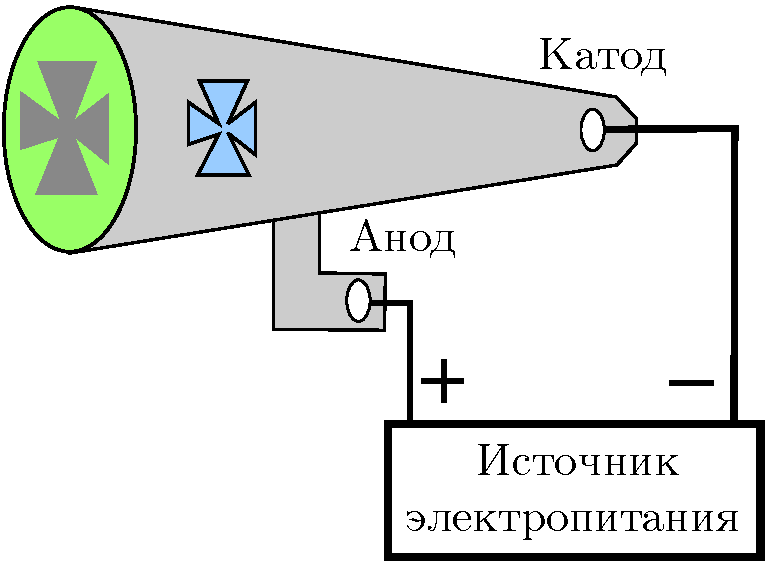
\includegraphics[width=5cm]{figs/how_it_started/crookes_tube.pdf}
    \caption{Трубка Крукса.}
    \label{fig:crookes_tube}
\end{figure}

Томсон исследовал обнаруженные лучи и установил, что они могут отклоняться электрическим полем (в дополнение к уже известному факту отклонения магнитным полем). Он пришёл к выводу, что эти лучи не являются формой света, а состоят из очень лёгких отрицательно заряженных частиц~--- электронов.

Он измерил отношение массы к заряду ($m/e$) для электрона и обнаружил, что оно примерно в 1800 раз меньше, чем у водорода, самого лёгкого известного атома. Это были частицы, не похожие ни на какие другие, известные ранее.

Томсон предположил, что атом не является неделимой частицей и что электроны~--- одна из составляющих его частей, что электроны существуют внутри атомов, а электрический ток~--- это не что иное, как электроны, перескакивающие с одного атома на соседний.

Логично было предположить и то, что для уравновешивания отрицательного заряда электронов и удержания их вместе должен существовать соизмеримый положительный заряд.

Не имея представления о том, откуда берётся этот положительный заряд, Томсон предположил, что положительный заряд находится внутри атома, и для простоты посчитал его сферичным.

\begin{figure}[htbp]
    \centering
    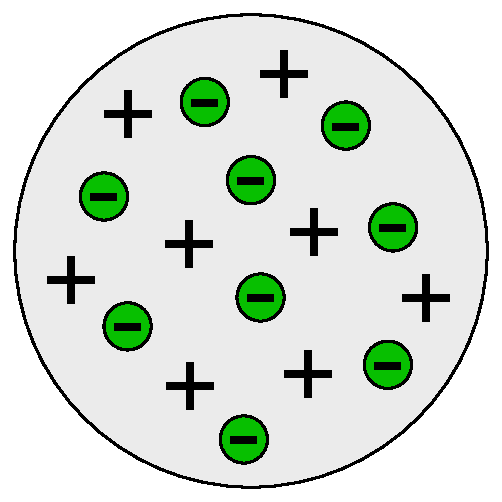
\includegraphics[width=3cm]{figs/how_it_started/plum_pudding.pdf}
    \caption{Модель сливового пудинга.}
    \label{fig:plum_pudding}
\end{figure}

Томсон также предположил, что электростатические силы распределяют электроны по этой сфере более или менее равномерно. Электроны могут перемещаться внутри этой сферы и, в связи с этим, он сравнил вещество сферы атома с жидкостью.

В рассуждениях учёного эта описанная положительная сфера была скорее абстракцией, чем каким-то материальным круглым объектом. Он не предлагал существование положительно заряженной субатомной частицы, аналогичной электрону.

Томсон назвал свою модель атома \textbf{моделью сливового пудинга}\label{term:plum_pudding}\index{модель сливового пудинга} (рис.~\ref{fig:plum_pudding}), поскольку электроны находились в положительном заряде, как изюм в сливовом пудинге.

\subsection*{Открытие $\alpha$-частиц}

В 1899~г. Эрнест Резерфорд открыл $\alpha$-частицы в ходе специального эксперимента для определения состава радиоактивного излучения.

Суть его опыта заключалась в следующем: свинцовый контейнер с солью радия (или другим радиоактивным препаратом) имел специальное окно, через которое излучение попадает на фотопластинку (рис.~\ref{fig:rutherford_experiment}).

Если в излучении имеются заряженные частицы, то, создав на их пути магнитное поле, можно отклонить траектории их движения. В результате след на фотопластинке будет сдвинут.

\begin{figure}[htbp]
    \centering
    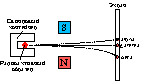
\includegraphics[width=7cm]{figs/how_it_started/rutherford_experiment.pdf}
    \caption{Эксперимент Резерфорда, который привёл к открытию $\alpha$-частиц.}
    \label{fig:rutherford_experiment}
\end{figure}

В результате на пластинке образуются три области. Две области были смещены в противоположных направлениях на разные расстояния, а на линии прямого воздействия тоже имелась засвеченная область. Это указывало на то, что в радиоактивном излучении присутствовали частицы трёх видов:

\begin{enumerate}[label=\arabic*)]
    \item Пятно с небольшим сдвигом оставляют тяжёлые положительные частицы (их и назвали \textbf{$\alpha$-частицами}\label{term:alpha_particle}\index{$\alpha$-частицы}).
    \item Пятно с большим противоположным сдвигом~--- лёгкие отрицательные \textbf{$\beta$-частицы}\label{term:beta_particle}\index{$\beta$-частицы} (электроны).
    \item Частицы, образовавшие пятно на прежнем месте,~--- электрически нейтральны. Это было \textbf{$\gamma$-излучение}\label{term:gamma_radiation}\index{$\gamma$-излучение}~--- электромагнитное излучение с высокой энергией.
\end{enumerate}

В 1906 году, изучая, как пучки $\alpha$-частиц отклоняются в магнитных и электрических полях, Резерфорд пришёл к выводу, что это, по сути, атомы гелия, лишённые двух электронов. В то время Томсон и Резерфорд мало что знали о внутренней структуре $\alpha$-частиц.

Модель Томсона в целом соответствовала имевшимся на тот момент экспериментальным данным. Томсон изучал $\beta$-частицы, которые отклонялись (рассеивались) на довольно малые углы, проходя через вещество.

Томсон рассуждал так: каждое взаимодействие частицы с электронами атома и положительной фоновой сферой приводит к незначительному отклонению, но сумма таких столкновений может быть значительной, если слой вещества будет довольно большим. Предполагалось, что рассеяние $\alpha$-частиц будет аналогичным. Однако\ldots

\subsection*{Опыты с золотой фольгой и планетарная модель атома}

В ходе эксперимента, проведённого в 1909 году, Ханс Гейгер и Эрнест Марсден обнаружили необъяснимое. Металлическая фольга рассеивала некоторые $\alpha$-частицы во всех направлениях, и даже иногда более чем на \ang{90} (рис.~\ref{fig:gold_foil}).

\begin{figure}
    \centering
    \begin{minipage}[t]{0.45\textwidth}
        \centering
        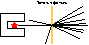
\includegraphics[width=5.5cm]{figs/how_it_started/gold_foil.pdf}
        \caption{Эксперимент с золотой фольгой.}
        \label{fig:gold_foil}
    \end{minipage}
    \hfill
    \begin{minipage}[t]{0.45\textwidth}
        \centering
        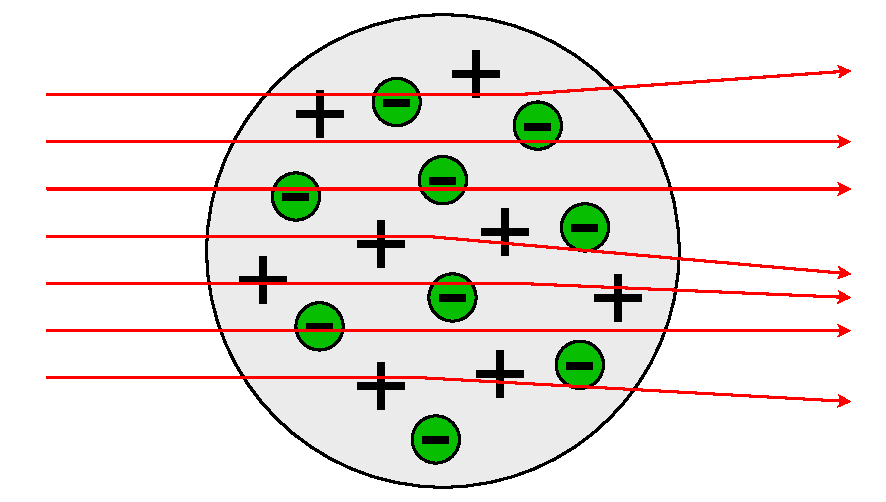
\includegraphics[width=4.5cm]{figs/how_it_started/incongruity.pdf}
        \caption{Так должны были бы вести себя $\alpha$-частицы при бомбардировании атома согласно модели сливового пудинга.}
        \label{fig:incongruity}
    \end{minipage}
\end{figure}

В этом эксперименте очень тонкая золотая фольга бомбардировалась $\alpha$-частицами. При этом большая часть частиц пролетала свободно сквозь фольгу, а некоторая часть отклонялась от первоначальной траектории. Однако были и частицы, которые не просто отклонялись, а меняли направление на близкое к противоположному (по сути, отражались фольгой).

Согласно модели Томсона, это было невозможно, так как все $\alpha$-частицы должны были проходить насквозь, либо незначительно отклоняться из-за взаимодействия с размытым положительным зарядом (рис.~\ref{fig:incongruity}).

В модели атома Томсона сфера положительного заряда, заполняющая атом и окружающая электроны, проницаема, а электроны могут перемещаться внутри неё. Следовательно, $\alpha$-частица может пройти через эту сферу, если это позволяют электростатические силы.

Более того, $\alpha$-частицы обычно обладают гораздо большей скоростью, чем $\beta$-частицы, то есть большей энергией и должны ещё меньше рассеиваться в аналогичных условиях.

Наблюдаемое заставило Резерфорда пересмотреть модель атома. Проблема модели Томсона заключалась в том, что положительный заряд атома был слишком рассредоточен, чтобы создавать достаточно сильную электростатическую силу, вызывающую наблюдаемое отталкивание.

Резерфорд посчитал, что положительный заряд не заполняет весь объём атома, а образует крошечное ядро, которое как минимум в \num{10000} раз меньше атома в целом. Весь этот положительный заряд, сосредоточенный в таком маленьком объёме, создаёт гораздо более сильное электрическое поле вблизи себя.

Ядро также несёт на себе подавляющую часть массы атома. Это означает, что оно может отклонять $\alpha$-частицы на угол до \ang{180} в зависимости от того, насколько близко с ядром они пролетают. Однако поскольку размер ядер очень мал, то и вероятность столкновения ядер не такая высокая, чтобы все $\alpha$-частицы отклонялись обратно.

Электроны окружают ядро, распределяясь по всему объёму атома. Поскольку их отрицательный заряд рассредоточен, а их общая масса невелика, они оказывают незначительное влияние на $\alpha$-частицу. Резерфорд предположил, что электроны вращаются по круговым орбитам вокруг ядра, подобно тому, как планеты вращаются вокруг Солнца. Данная модель строения атома получила название \textbf{планетарной модели}\label{term:planetary_model}\index{планетарная модель атома} (рис.~\ref{fig:planetary_model}).

\begin{figure}[htbp]
    \centering
    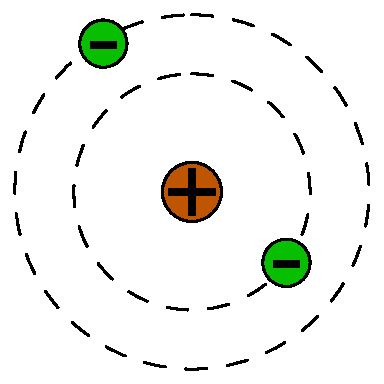
\includegraphics[width=2.5cm]{figs/how_it_started/planetary_model.pdf}
    \caption{Планетарная модель атома Резерфорда.}
    \label{fig:planetary_model}
\end{figure}

Чтобы проверить свои предположения, Резерфорд разработал математическую модель, которая позволяла предсказать энергию $\alpha$-частиц при различных углах их рассеяния при выходе из золотой фольги. И эта модель действительно верно предсказала данные, подтверждённые в ходе эксперимента, проведённого в 1913 году.

В итоге планетарная модель атома объясняла как результаты $\beta$-расщепления, полученные Томсоном, так и результаты $\alpha$-расщепления, полученные Гейгером и Марсденом.

\subsection*{Открытие протонов и нейтронов}

В 1917 году Резерфорд бомбардировал азот $\alpha$-частицами и наблюдал, как из газа испускаются ядра водорода (Резерфорд сумел распознать их, потому что он ранее с ними уже сталкивался, бомбардируя водород $\alpha$-частицами и наблюдая атомы водорода в продуктах).

Учёный пришёл к выводу, что ядра водорода возникли из ядер самих атомов азота. Фактически, это была ядерная реакция расщепления азота.

Из своей собственной работы и работ своих учеников Нильса Бора и Генри Мозли Резерфорд знал, что положительный заряд любого атома всегда можно количественно приравнять к заряду целого числа ядер водорода. Это, вкупе с атомной массой многих элементов, примерно эквивалентной массе целого числа атомов водорода, которые тогда считались легчайшими частицами, привело его к выводу, что ядра водорода были единичными частицами и основной составляющей всех атомных ядер. Он назвал такие частицы \textbf{протонами}.

Дальнейшие эксперименты Резерфорда показали, что ядерная масса большинства атомов больше, чем сумма масс протонов, которыми они обладают. Следовательно, эта избыточная масса должна состоять из ранее неизвестных нейтрально заряженных частиц, которые предварительно назвали \textbf{нейтронами}.

В 1928 году Уолтер Боте заметил, что бериллий испускает электрически нейтральное излучение с большой проникающей способностью при бомбардировке его $\alpha$-частицами. Позже было обнаружено, что происходит эмиссия протонов из парафина, если подвергнуть его воздействию данного излучения (рис.~\ref{fig:discovery_of_neutrons}).

\begin{figure}[htbp]
    \centering
    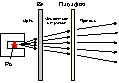
\includegraphics[width=6.5cm]{figs/how_it_started/discovery_of_neutrons.pdf}
    \caption{Эксперимент, в ходе которого был открыт нейтрон.}
    \label{fig:discovery_of_neutrons}
\end{figure}

Первоначально считалось, что это $\gamma$-излучение высокой энергии, поскольку $\gamma$-излучение оказывает аналогичное влияние на электроны в металлах, но Джеймс Чедвик обнаружил, что эффект ионизации был слишком сильным, чтобы быть вызванным электромагнитным излучением.

В 1932 году Чедвик подвергал различные химические элементы, такие как водород и азот, загадочному <<излучению бериллия>> и, измеряя энергии выбитых протонов, пришёл к выводу, что это излучение на самом деле состоит из электрически нейтральных частиц, которые не могут быть безмассовыми как $\gamma$-лучи.

При этом данные частицы обладают массой, аналогичной массе протона. Данные частицы были объявлены нейтронами Резерфорда.

Нейтроны обладают самой высокой проникающей способностью из описанных частиц, поскольку не имеют заряда и обладают высокой скоростью (рис.~\ref{fig:neutron_penetration}). Задержать их могут либо специальные вещества-поглотители, либо довольно толстые слои материалов.

\begin{figure}[htbp]
    \centering
    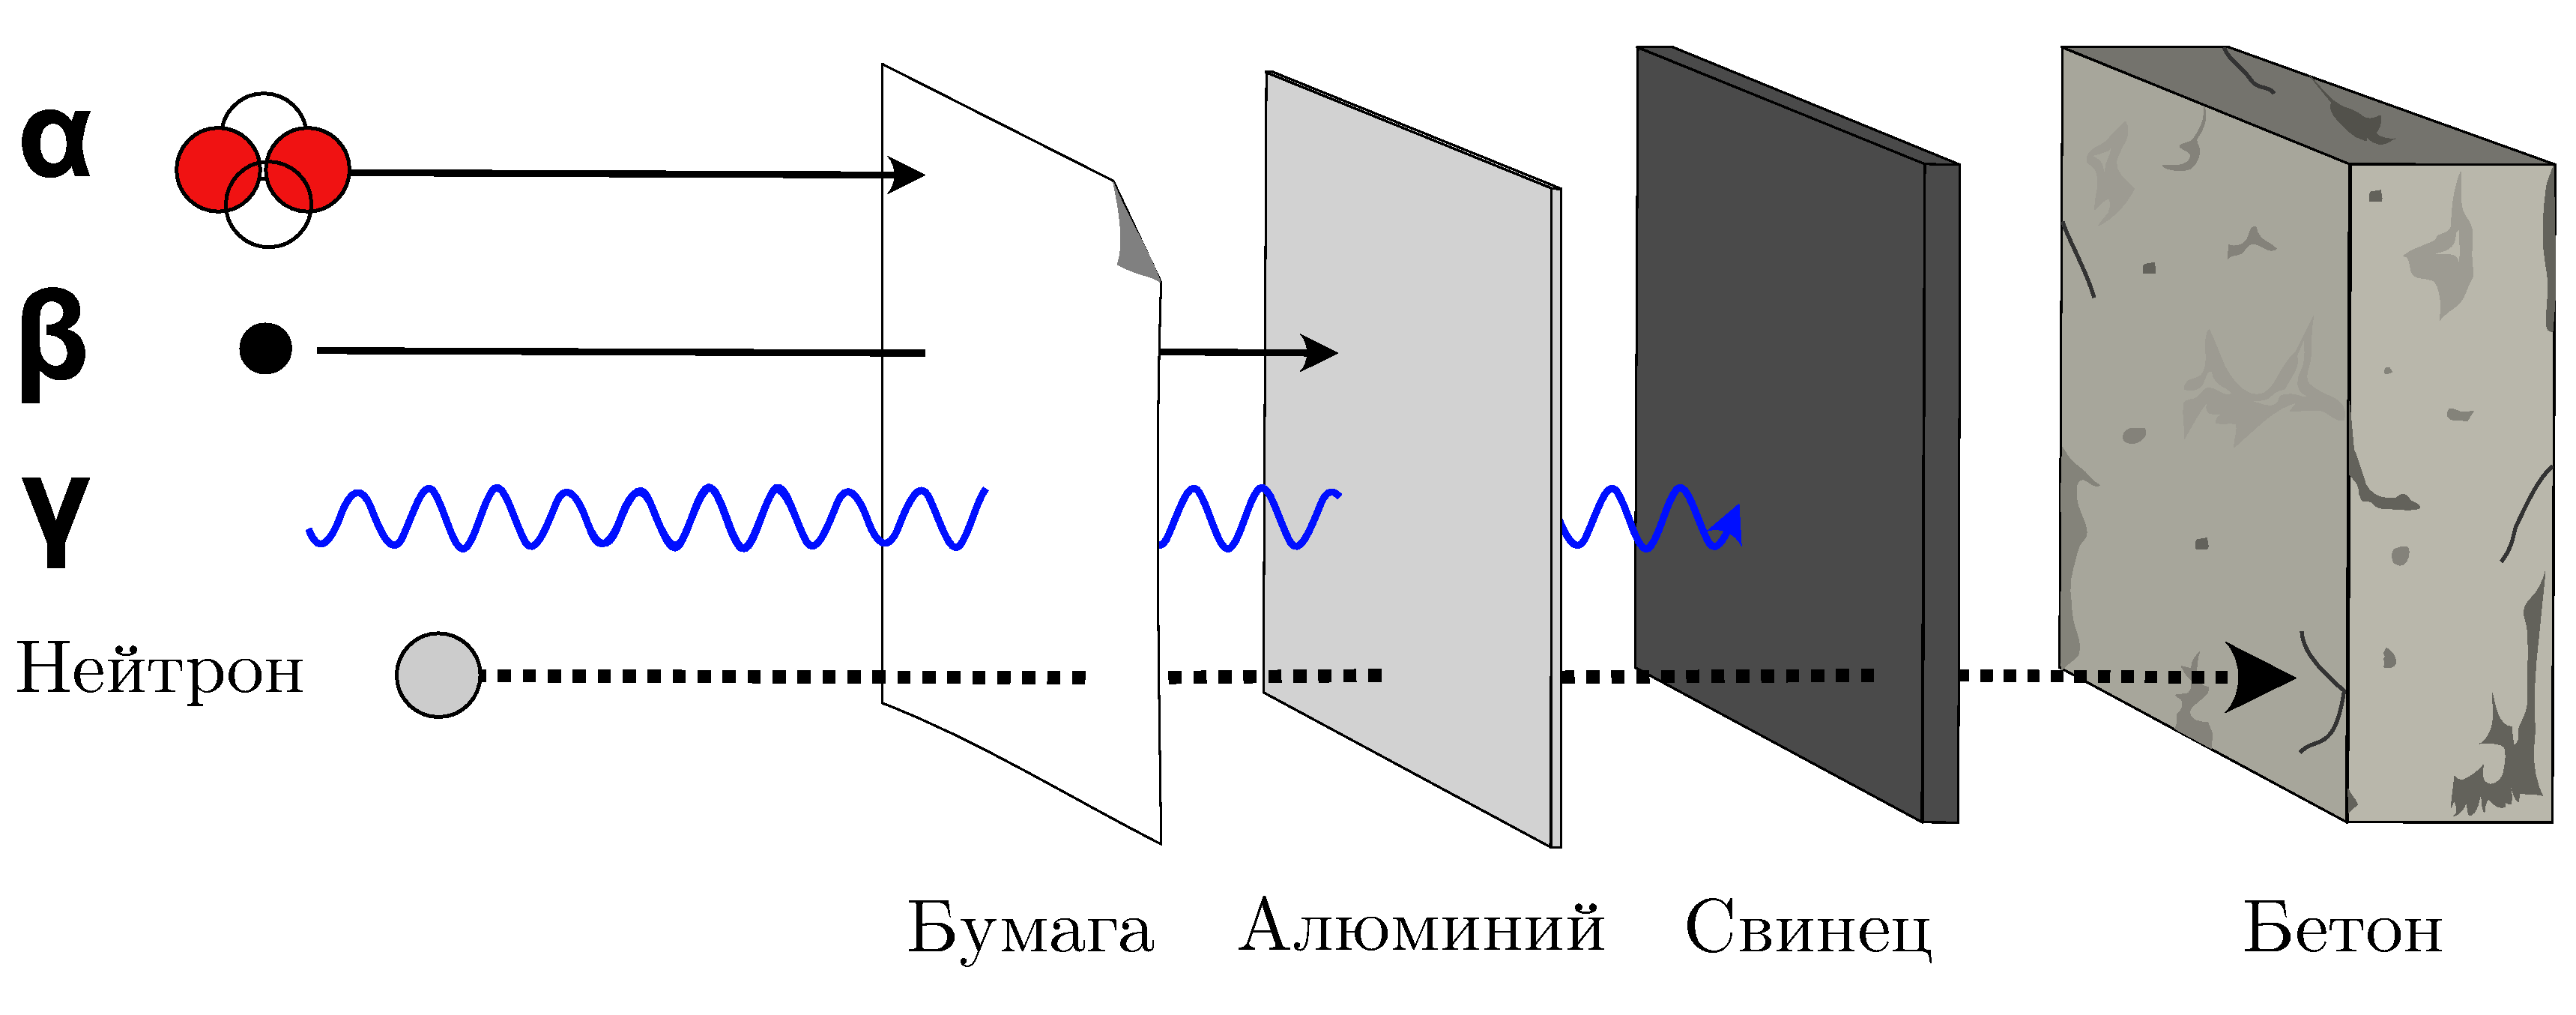
\includegraphics[width=9cm]{figs/how_it_started/neutron_penetration.pdf}
    \caption{Нейтроны обладают огромной проникающей способностью, в отличие от многих других элементарных частиц.}
    \label{fig:neutron_penetration}
\end{figure}

\subsection*{Квантовая модель Бора и дальнейшее развитие}

Планетарная модель Резерфорда хорошо объясняла наблюдаемые эксперименты, но не выдерживала никакой критики с точки зрения законов физики, поскольку содержала проблему устойчивости: по законам классической физики электроны, вращаясь вокруг ядра, должны были излучать энергию и падать на ядро. Однако мы знаем, что большинство атомов стабильно.

Датский физик Нильс Бор в 1913 году предложил \textbf{квантовую модель атома}\label{term:quantum_model_of_the_atom}\index{квантовая модель атома}, основанную на идеях Макса Планка и Альберта Эйнштейна. Основные постулаты Бора:

\begin{itemize}
    \item Электроны могут находиться только на определённых дискретных орбитах, соответствующих квантовым уровням энергии.
    \item При переходе электрона с одной орбиты на другую излучается или поглощается квант энергии.
\end{itemize}

Модель Бора хорошо объясняла спектральные линии водорода\footnote{При нагреве водорода он излучает узкие, строго определённые диапазоны длин волн.} и стала важным шагом в развитии квантовой механики. В то время уже стало понятно, что законами классической физики состояние атома не описать.

Дальнейшие работы Эрвина Шрёдингера и Вернера Гейзенберга в 20-х годах привели к созданию волновой механики, где электроны описываются как облака с определённой плотностью вероятности нахождения в той или иной точке, а не как частицы на фиксированных орбитах.

В конечном итоге научная эволюция привела нас к квантовому пониманию строения атома и даже мира в целом. Квантовано оказалось многое: энергия в атомах, угловой момент электронов, другие физические величины. Именно с этой точки зрения стоит рассматривать свойства и изучать атомы и молекулярные системы. 

Математический аппарат квантовой механики довольно громоздкий и труден для понимания, поэтому выходит за рамки данного учебника. Однако не всё так плохо. С точки зрения химика достаточно иметь общие представления о законах квантовой физики, поскольку на практике всё обычно упрощается до хорошо понимаемых и схематизированных абстрактных понятий.

Сформулируйте понятия из потока терминов на основании прочитанного в этом разделе.

\begin{termlist}
    \hyperref[term:systematic_thinking]{Системное мышление}, 
    \hyperref[term:plum_pudding]{модель сливового пудинга}, 
    \hyperref[term:alpha_particle]{$\alpha$-частицы}, 
    \hyperref[term:beta_particle]{$\beta$-частицы}, 
    \hyperref[term:gamma_radiation]{$\gamma$-излучение}, 
    \hyperref[term:planetary_model]{планетарная модель атома}, 
    \hyperref[term:quantum_model_of_the_atom]{квантовая модель атома}.
\end{termlist}

\begin{problem}{}{how_it_started2}
    Составьте таблицу сравнений трёх моделей атома:
    \begin{itemize}
        \item модель Томсона («сливовый пудинг»);
        \item планетарная модель Резерфорда;
        \item квантовая модель Бора.
    \end{itemize}

    Для каждой модели укажите:
    \begin{itemize}
        \item как расположены электроны;
        \item какие экспериментальные данные подтверждали модель.
    \end{itemize}

    \begin{sol}{\ref{prob:how_it_started2}}
        \begin{table}[ht]
            \small
            \begin{tabularx}{\textwidth}{
                >{\hsize=1\hsize}Y
                >{\hsize=1\hsize}Y
                >{\hsize=1\hsize}Y
                >{\hsize=1\hsize}Y
                }
                \hline
                \rowcolor{green!5}
                Критерий & Модель Томсона & Модель Резерфорда & Модель Бора \\
                \hline
                Расположение электронов & Равномерно распределены в положительной сфере. & Движутся по орбитам вокруг ядра & На дискретных квантовых орбитах \\
                \hline
                Подтверждающие эксперименты & Отклонение катодных лучей в полях (Томсон) & Рассеяние $\alpha$-частиц на золотой фольге (Гейгер, Марсден) & Спектральные линии водорода \\
                \hline
            \end{tabularx}
        \end{table}
    \end{sol}
\end{problem}

\begin{problem}{}{how_it_started3}
    Сформулируйте противоречие модели атома Томсона и результатов экспериментов с золотой фольгой.

    \begin{sol}{\ref{prob:how_it_started3}}
        Распределение заряда. В модели Томсона положительный заряд был равномерно распределён по всему объёму атома, а значит, электрическое поле внутри атома не могло вызвать сильного отклонения $\alpha$-частиц, а тем более кардинально изменить их траекторию.
            
        Наблюдаемые резкие отклонения указывали на наличие в атоме точечного источника сильного кулоновского отталкивания~--- ядра с большим положительным зарядом.
    \end{sol}
\end{problem}

\begin{problem}{}{how_it_started4}
    Почему открытие нейтронов стало необходимым после установления планетарной модели атома?

    \begin{sol}{\ref{prob:how_it_started4}}
        Чтобы решить <<проблему массы>>, ведь масса большинства исследуемых атомов превышала сумму масс составляющих их протонов. Например, ядро гелия было вдвое тяжелее, чем масса двух протонов. Разница требовала нейтральных частиц.
    \end{sol}
\end{problem}

Очень часто важно думать не о том, что подтверждает то или иное утверждение, а о том, что оно \emph{не} подтверждает.

Это связано со склонностью человека к \textbf{предвзятости подтверждения}~--- желанием использовать новую информацию для подтверждения уже имеющихся взглядов, но не для того, чтобы их опровергнуть.

Полностью избежать предвзятости подтверждения нельзя, это связано с особенностями работы нашего мышления. Все мы придерживаемся определённых взглядов и нельзя относиться скептически абсолютно ко всему. Но можно научить себя смотреть на вещи критически.

\begin{problem}{}{how_it_started5}
    $\bigstar$ \textit{Профессор Недоумелкин} посетил лабораторию Резерфорда и после ознакомления с моделью Томсона и результатами опытов с золотой фольгой заявил, что он объявляет свою гипотезу о строении атома:

    \medskip

    \emph{Я уверен, вы все заблуждаетесь! Атом имеет слоистую структуру! Положительные и отрицательные слои чередуются! $\alpha$-частицы отражаются от границ слоёв, если попадают в <<узкие зоны>>.}

    \medskip

    Опровергните доводы профессора.

    \begin{sol}{\ref{prob:how_it_started5}}
        Гипотеза Недоумелкина несостоятельна потому что:
        \begin{itemize}
            \item Гипотеза слоистой структуры предполагает регулярные отражения от каждого слоя из-за их большого количества, а не редкое катастрофическое рассеяние. Наблюдаемая статистика несовместима с равномерным распределением слоёв.
            \item Чтобы отразить тяжёлую $\alpha$-частицу, граница слоя должна создавать колоссальное электрическое поле. В модели Томсона даже равномерное распределение заряда не давало такого эффекта. Чередующиеся слои усилили бы поле лишь незначительно (за счёт суперпозиции), но не в тысячи раз, как требовалось для обратного рассеяния.
            \item Такая структура должна быть нестабильна из-за стремления к схлопыванию при притяжении разноимённо заряженных слоёв и иметь сильные внутренние напряжения из-за отталкивания одноимённо заряженных.
            \item Нет <<тени>> от слоёв. Если бы слои существовали, $\alpha$-частицы, проходящие сквозь них, должны были бы замедляться из-за притяжения/отталкивания и создавать характерную интерференционную картину на детекторе. На деле большинство частиц пролетали без потери энергии и отклонения~--- это возможно только если большая часть атома <<пуста>>, а не заполнена слоями.
        \end{itemize}
    \end{sol}
\end{problem}

\clearpage

\section{Атомное ядро}

\hspace*{\parindent}Атом состоит из положительно заряженного \textbf{атомного ядра}\label{term:atomic_nucleus}\index{атомное ядро} и отрицательно заряженных \textbf{электронов}\label{term:electron}\index{электрон}, находящихся возле ядра и связанных с ним. Как мы уже узнали, атомное ядро имеет очень небольшие размеры относительно общего размера атома, однако содержит в себе практически всю массу атома\footnote{Масса протона $m_p \approx \qty{1,6726e-27}{\kg}$, масса электрона $m_e \approx \qty{9,11e-31}{\kg}$, т.~е. протон тяжелее электрона в \num{1836} раз. Размер атомного ядра порядка \qty{e-15}{\m}, размер атома порядка \qty{e-10}{\m}, разница пять порядков.}.

Ядра атомов химических элементов состоят из \textbf{нуклонов}, всего двух типов~--- положительно заряженных \textbf{протонов} $p$ и незаряженных \textbf{нейтронов} $n$. Например, ядро атома водорода состоит всего из одного протона, а ядро гелия~--- из четырёх нуклонов: двух протонов и двух нейтронов (Рис~\ref{fig:H-He-Li}).

Ядро лития состоит из трёх протонов и четырёх нейтронов. Как видите, без последних не обходится. Всё дело в том, что нейтроны нужны для стабилизации атомного ядра. Чем больше ядро, тем больше нужно нейтронов.

\begin{figure}[htbp]
    \centering
    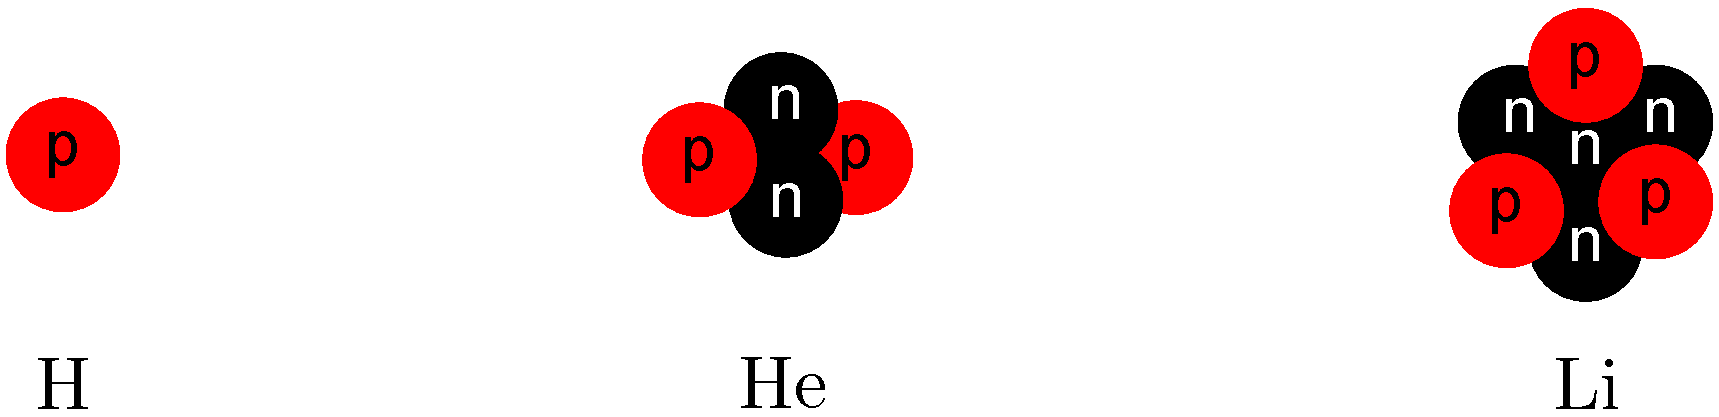
\includegraphics[width=9cm]{figs/atomic_nucleus/H-He-Li.pdf}
    \caption{Состав ядер химических элементов: гелия, лития и водорода.}
    \label{fig:H-He-Li}
\end{figure}

Каждый последующий элемент отличается от предыдущего тем, что у него на один протон в ядре больше. Разумеется, вы уже догадались, как для любого элемента из периодической таблицы определить количество протонов в его ядре~--- это просто его номер в таблице.

\subsection*{Характеристики атомного ядра}\label{sec:nuclear_numbers}

Для того чтобы описать состав атомного ядра используют три числа~--- \textbf{зарядовое}\label{term:atomic_number}\index{зарядовое число}, \textbf{массовое}\label{term:mass_number}\index{массовое число} и \textbf{число нейтронов}\label{term:neutron_number}\index{число нейтронов}. Ознакомьтесь с табл.~\ref{tab:nuclear_numbers}, и вам многое станет понятно.

\begin{table}
    \small
    \caption{Числа, характеризующие состав атомного ядра}
    \label{tab:nuclear_numbers}
    \begin{tabularx}{\textwidth}{
        >{\hsize=0.9\hsize}Y
        >{\hsize=0.8\hsize}Z
        >{\hsize=1\hsize}Y
        >{\hsize=1\hsize}Y
        >{\hsize=1.3\hsize}Y
        }
        \hline
        \rowcolor{green!5}
        Название\newline числа & Обо\-зна\-че\-ние & Что \newline показывает & Как\newline записывается & Примечание \\
        \hline
        Зарядовое & $Z$ & Количество протонов в ядре & Нижним индексом перед символом элемента: \ce{_8O} & Равно номеру элемента в периодической системе. Равно количеству электронов у нейтрального атома \\
        \hline
        Массовое & $A$ & Суммарное количество нуклонов (протонов + нейтронов) в ядре & Верхним индексом перед символом элемента: \ce{^16O} & Позволяет оценить массу атома. Позволяет различать изотопы \\
        \hline
        Число \newline нейтронов & $N$ & Количество нейтронов в ядре & Обычно не записывается & Позволяет различать изотопы \\
        \hline
    \end{tabularx}
\end{table}

По определению, все три числа связаны простым соотношением \ref{eq:nuclear_numbers}:

\begin{equation}
    \label{eq:nuclear_numbers}
    \fbox{$N = A - Z$}.
\end{equation}

Давайте условимся, что здесь и далее важные формулы мы будем отмечать рамкой. Эти соотношения вам нужно знать обязательно! 

По сути, зарядовое число $Z$ показывает, \emph{какой это химический элемент}, что и так можно понять из его буквенного обозначения, поэтому запись вроде \ce{_8O} обычно никогда не используется: достаточно просто <<\ce{O}>>. При этом ясно, что речь идёт о кислороде, а значит его зарядовое число равно восьми.

Поскольку атом в целом электронейтрален, положительный заряд его атомного ядра должен уравновешиваться противоположным по знаку и равным по величине зарядом электронов. Поэтому число протонов в ядре равно количеству электронов в нейтральном атоме.

\subsection*{Изотопы}

В отличие от зарядового числа $Z$, число нейтронов ($N$) в атомах одного и того же химического элемента может быть разным. Например, известно о существовании трёх видов атомов водорода с разными массовыми числами (рис.~\ref{fig:hydrogen_isotopes}).

Самый лёгкий тип атомов водорода называется \textbf{протий}\label{term:protium}\index{протий} (\ce{H})~--- такие атомы наиболее распространены в природе. У протия ядро представляет собой просто один протон. Другой, более тяжёлый водород, называют \textbf{дейтерий}\label{term:deuterium}\index{дейтерий} (\ce{D})~--- у него ядро состоит из одного протона и одного нейтрона. Наконец, самый тяжёлый водород называют \textbf{тритий}\label{term:tritium}\index{тритий} (\ce{T})~--- его ядро атома состоит из одного протона и двух нейтронов\footnote{Протий составляет > \qty{99,98}{\percent} всех атомов водорода во Вселенной. Дейтерий устойчив, в воде на Земле его атомов содержится примерно \qty{0,0156}{\percent}. Тритий не устойчив и в природе хотя и встречается (образуется в верхних слоях атмосферы под действием космических лучей), но в крайне малых количествах.}.

\begin{figure}[htbp]
    \centering
    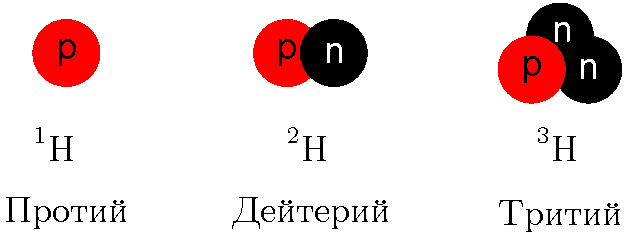
\includegraphics[width=5.5cm]{figs/atomic_nucleus/hydrogen_isotopes.pdf}
    \caption{Изотопы водорода.}
    \label{fig:hydrogen_isotopes}
\end{figure}

Атомы одного химического элемента, отличающиеся только числом нейтронов, называются \textbf{изотопами}\label{term:isotope}\index{изотоп} или \textbf{нуклидами}. То есть все изотопы одного химического элемента имеют одно и то же зарядовое число $Z$ и занимают одно и то же положение в периодической системе, но отличаются числами $A$ и $N$, то есть имеют разное количество нейтронов, но одинаковое количество протонов.

Изотопы записывают с использованием массового числа $A$ используя два варианта. В первом варианте по-русски пишут название химического элемента, а затем через дефис~--- массовое число $A$, например, уран-235, уран-238. Другой, более компактный вариант~--- использовать буквенное обозначение элемента, а массовое число показать верхним левым индексом: \ce{^235U}, \ce{^238U}.

Ещё раз обратите внимание, что оба эти изотопа представляют собой один и тот же химический элемент~--- уран.

Другой пример~~--- углерод-12, углерод-13 и углерод-14 представляют собой три изотопа углерода с массовыми числами 12, 13 и 14 соответственно. Атомный номер углерода равен 6, поэтому в каждом из этих изотопов ядро содержит 6 протонов, а число нейтронов в этих изотопах составляет 6, 7 и 8 соответственно.

Давайте решим пару задач.

\begin{problem}{}{atomic_nucleus1}
    Для нуклонов \ce{^18O}, \ce{^31P}, \ce{^66Zn} и \ce{^202Hg} найдите массовые, зарядовые числа и число нейтронов.

    \begin{sol}{\ref{prob:atomic_nucleus1}}
        Массовое число уже указано в названии нуклона верхним левым индексом, т.~е.\\
        для \ce{^18O} $A = 18$,\\
        для \ce{^31P} $A = 31$,\\
        для \ce{^66Zn} $A = 66$,\\
        для \ce{^202Hg} $A = 202$.

        Зарядовые числа найдём по номеру химических элементов в \hyperref[appendix:periodic_table]{периодической таблице}:\\
        для \ce{^18O} $Z = 8$,\\
        для \ce{^31P} $Z = 15$,\\
        для \ce{^66Zn} $Z = 30$,\\
        для \ce{^202Hg} $Z = 80$.

        Число нейтронов $N$ найдём по разности массового и зарядового числа $N = A - Z$:\\ 
        для \ce{^18O} $N = 18 - 8 = 10$,\\
        для \ce{^31P} $N = 31 - 15 = 16$,\\
        для \ce{^66Zn} $N = 66 - 30 = 36$,\\
        для \ce{^202Hg} $N = 202 - 80 = 122$. 
    \end{sol}
\end{problem}

\begin{problem}{}{atomic_nucleus2}
    Ядро атома некоторого элемента содержит 46 нейтронов, а электронная оболочка~--- 34 электрона. Что это за элемент? О каком изотопе идёт речь?

    \begin{sol}{\ref{prob:atomic_nucleus2}}
        Количество электронов численно равно количеству протонов и зарядовому числу атомного ядра, следовательно, для нашего элемента $Z = 34$. Зарядовое число равно номеру элемента в периодической системе, элемент с номером 34~--- это селен. Массовое число данного изотопа равно сумме зарядового числа и числа нейтронов $A = Z + N = 34 + 46 = 80$. Следовательно, это изотоп \ce{^80Se}. 
    \end{sol}
\end{problem}

\subsection*{Свойства изотопов}

Одинаковы или различны химические и физические свойства у изотопов? Изотопы имеют одинаковое электронное строение, и обычно небольшая разница в числе нейтронов почти не влияет на \emph{химические} свойства элементов.

Однако это не всегда так. Для самых лёгких элементов, например, водорода~--- изотопы сильно различаются по массе. Например, дейтерий в два раза тяжелее протия, а тритий тяжелее в целых три раза. Из-за этого поведение изотопов начинает различаться, к примеру, в скоростях химических реакций. Эти явления называют \textbf{изотопными}\label{term:isotopic_effect}\index{изотопный эффект} эффектами.

\emph{Физические} же свойства изотопов могут довольно сильно различаться, потому что изотопы часто сильно различаются по стабильности, а вещества имеющие в своём составе разные изотопы обладают разными физическими свойствами. В табл.~\ref{tab:water_isotopes_physical_properties} вы можете сравнить некоторые физические свойства обычной и тяжёлой воды.

\begin{table}[htbp]
    \small
    \caption{Различие физических свойств обычной и тяжёлой воды.}
    \label{tab:water_isotopes_physical_properties}
    \begin{tabularx}{\textwidth}{
        >{\hsize=1.6\hsize}Y
        >{\hsize=0.7\hsize}Z
        >{\hsize=0.7\hsize}Z
        }
        \hline
        \rowcolor{green!5}
        Физические свойства (при н.~у.) & \ce{H2O} & \ce{D2O} \\
        \hline
        Плотность, $\text{г}/\text{см}^3$ & \num{1,0000} & \num{1,1059} \\
        $\mathrm{t_{\text{кип}}}$, \unit{\degreeCelsius} & 100 & \num{101.4} \\
        $\mathrm{t_{\text{пл}}}$, \unit{\degreeCelsius} & 0 & \num{3,8} \\
        \hline
    \end{tabularx}
\end{table}

\subsection*{Стабильность изотопов}

Некоторые изотопы являются радиоактивными, то есть распадаются с течением времени и поэтому называются \textbf{радиоизотопами}\label{term:radioisotope}\index{радиоизотоп} или \textbf{радионуклидами}.

Изотопы, которые не распадаются с течением времени, называются \textbf{стабильными изотопами}\label{term:stable_isotope}\index{стабильный изотоп}. Например, \ce{^14C} представляет собой радиоактивную форму углерода, а \ce{^12C} и \ce{^13C}~--- стабильные изотопы. Нетрудно догадаться, что именно такие изотопы преобладают на Земле и в Солнечной системе.

Стабильность изотопов можно оценить при помощи такого показателя, как \textbf{период полураспада}\label{term:half-life}\index{период полураспада} ($T_{1/2}$). Это время, за которое распадается половина образца вещества в результате радиоактивного распада. Чем меньше период полураспада изотопа, тем он менее стабилен и более радиоактивен.

\begin{figure}[htbp]
    \centering
    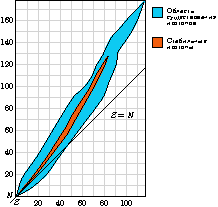
\includegraphics[width=9cm]{figs/atomic_nucleus/isotope_stability.pdf}
    \caption{Стабильность изотопов. Ядру атома необходимо определённое число нейтронов для стабилизации.}
    \label{fig:isotope_stability}
\end{figure}

Взгляните на график стабильности изотопов (рис.~\ref{fig:isotope_stability}). Примечательно, что область стабильных изотопов расходится с линией $Z = N$ с ростом зарядового числа. Как мы уже говорили, нейтроны необходимы для стабилизации протонов в атомном ядре.

С увеличением зарядового числа $Z$ требуется всё больше нейтронов для стабилизации ядра. Например, для \ce{^3He} соотношение нейтронов к протонам равно $1/2$, а для \ce{^238U} уже больше, чем $3/2$.

\ce{^40Ca} является самым тяжёлым стабильным нуклидом с равным числом нейтронов и протонов. Все стабильные нуклиды тяжелее него имеют больше нейтронов, чем протонов.

Все химические элементы с $Z > 92$ не имеют стабильных изотопов. Элементы с меньшим зарядовым числом имеют как стабильные изотопы, так и радионуклиды.

Однако отношение числа нейтронов к числу протонов~--- это не единственный фактор, определяющий ядерную стабильность. Большое влияние оказывает также \hyperref[tab:isotope_stability]{чётность или нечётность} чисел $Z$, $N$ и $A$. 

Нечётность как $Z$, так и $N$ приводит к снижению ядерной энергии связи, делая нечётные ядра, как правило, менее стабильными. Большинство стабильных нуклидов имеют чётное число протонов и чётное число нейтронов, то есть все числа $Z$, $N$ и $A$ чётные.

Существуют стабильные изотопы, в которых нечётно либо число протонов, либо число нейтронов. А вот устойчивые нуклиды, в которых и число протонов, и число нейтронов нечётное, встречаются крайне редко.

\begin{table}[htbp]
    \small
    \caption{Количество стабильных изотопов в зависимости от чётности и нечётности количества протонов и нейтронов в ядре.}
    \label{tab:isotope_stability}
    \begin{tabularx}{\textwidth}{
        >{\hsize=3.5\hsize}Y
        >{\hsize=0.5\hsize}Z
        >{\hsize=0.5\hsize}Z
        >{\hsize=0.5\hsize}Z
        >{\hsize=0.5\hsize}Z
        >{\hsize=0.5\hsize}Z
        }
        \hline
        \rowcolor{green!5}
        Чётность, $Z/N$ & ЧЧ & НН & ЧН & НЧ & Всего \\
        \hline
        Стабильные ($T_{1/2} > 4$ млрд лет) & 147 & 5 & 53 & 48 & 253 \\
        Долгоживущие ($\num{4e6} > T_{1/2} > \num{e5}$ лет) & 23 & 4 & 3 & 5 & 35 \\
        \hline
        Всего & 170 & 9 & 56 & 53 & 288 \\
        \hline
    \end{tabularx}
\end{table}

На Земле химические элементы обычно представляют собой смесь изотопов, например, природный хлор состоит на \qty{75,8}{\percent} из \ce{^35Cl} и на \qty{24,2}{\percent} из \ce{^37Cl}, поэтому среднюю массу атома, которая используется в практических расчётах, нужно определять с учётом фактического распределения изотопов в природном веществе.

В природе радионуклиды обычно распадаются в результате последовательной серии $\alpha$- и $\beta $-распадов, превращаясь по цепочке в различные изотопы. Давайте познакомимся с этими процессами.

При \textbf{$\alpha$-распаде} атомное ядро испускает $\alpha$-частицу (то есть ядро атома гелия). При этом массовое число $A$ уменьшается на 4, а зарядовое число $Z$ уменьшается на 2:

\reaction{
    \label{eq:alpha_decay}
    _$Z$^$A$X -> _$Z - 2$^$A - 4$Y + _2^4He{.}
}

При \textbf{$\beta$-распаде} (бета-минус-распад) атомное ядро испускает электрон и антинейтрино. При этом один нейтрон внутри ядра превращается в протон, зарядовое число увеличивается на 1, а массовое число не меняется:

\reaction{
    \label{eq:beta-minus-decay}
    _$Z$^$A$X -> _$Z + 1$^$A$Y + $e^{-}$ + ${\overline{\nu}}_e${.} 
}

На рис.~\ref{fig:decay_of_radon} приведён пример цепочки распада радона-222, речь о котором пойдёт ниже.

\begin{figure}
    \centering
    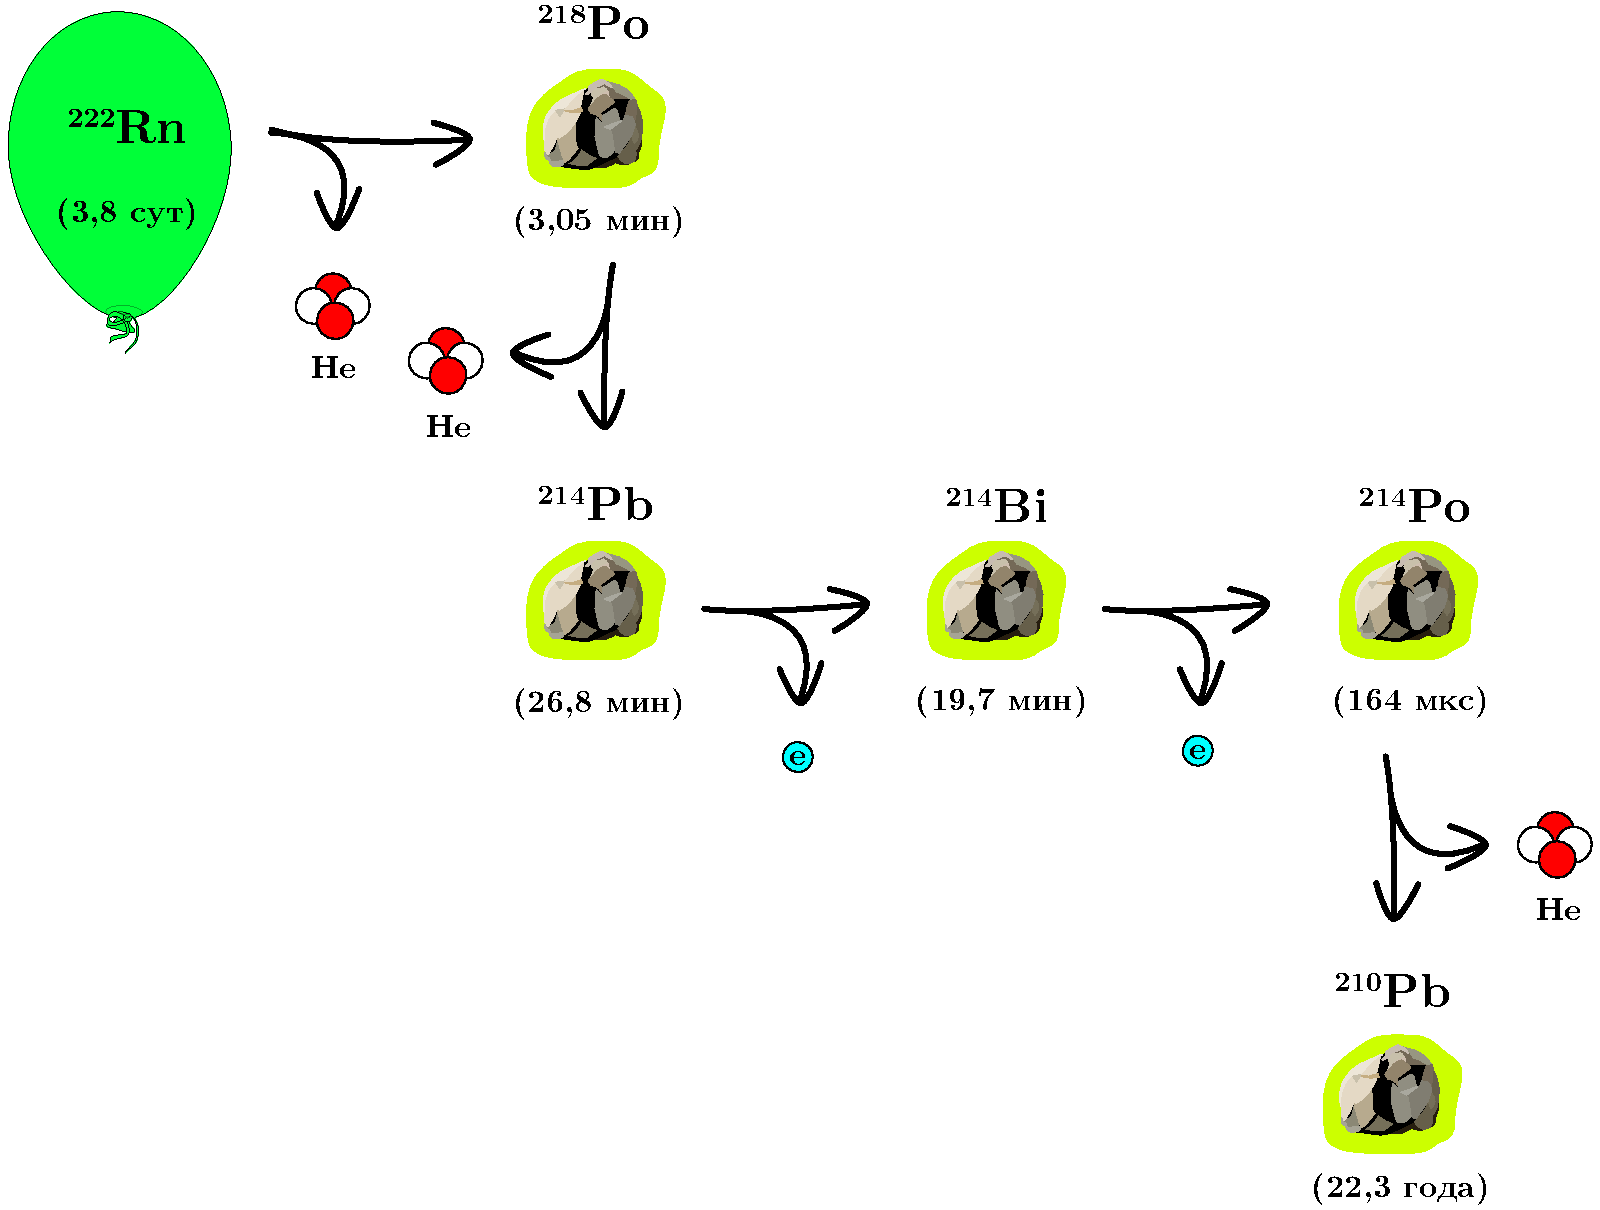
\includegraphics[width=9cm]{figs/atomic_nucleus/decay_of_radon.pdf}
    \caption{Ряд радиоактивного распада радона-222. Приведены периоды полураспада образующихся изотопов.}
    \label{fig:decay_of_radon}
\end{figure}

\subsection*{Радоновая опасность}

Расскажем о некоторых случаях, при которых человек сталкивается с радиоизотопами, либо использует их. Первый пример~--- это так называемая \textbf{радоновая опасность}\label{term:radon hazard}\index{радоновая опасность}: это широко распространённое радиоактивное поражение лёгких, вызванное попаданием в них радона-222 и продуктов его распада.

По статистике ВОЗ, от 3 до \qty{14}{\percent} всех случаев рака лёгких вызваны именно поражением радоном. Откуда он берётся? Если при строительстве домов используются материалы с высоким содержанием урана (особенно гранит), то в результате цепочки распада из него образуется радон и накапливается в трещинах и полостях материалов, а затем попадает в воздух:

\reaction*{^238U ->[-\alpha] ^234Th ->[-\beta] ^234Pa ->[-\beta] ^234U ->[-\alpha] ^230Th ->[-\alpha] ^226Ra ->[-\alpha] ^222Rn{.}}

При этом особенно страдают подвалы домов, поскольку они содержат большое количество необлицованных материалов, бетонных пустот и пр. Радон является тяжёлым газом, накапливающемся в низинах. Именно поэтому запрещено устраивать жилые помещения в цокольных этажах.

От региона к региону уровень риска радоновой опасности различается в связи с разным содержанием урана в природных материалах.

\subsection*{Радиоуглеродный анализ}\label{term:radiocarbon_dating}\index{радиоуглеродный анализ}

Это метод определения возраста органических материалов путём измерения содержания в них радиоактивного изотопа углерода-14 относительно стабильных изотопов углерода. Этим методом можно примерно определить возраст древних произведений искусства (например, подлинность картины), останков животных и т.~п.

Вот как всё происходит. В верхних слоях атмосферы под действием космических лучей азот-14 превращается в углерод-14:

\reaction*{^14N + $n$ -> ^14C + $p${.}}

Затем углерод-14 в составе углекислого газа включается в глобальный углеродный цикл. Растения усваивают углерод-14 в процессе фотосинтеза и накапливают его. При этом в них поддерживается постоянное соотношение изотопов углерод-14/углерод-12, точно такое же, как в атмосфере. Животные поедают растения, и углерод-12 мигрирует по пищевой цепочке.

После того как организмы гибнут, обмен углеродом с окружающей средой прекращается. Углерод-14 распадается, а стабильные изотопы сохраняются.

По остаточному содержанию углерода-14, зная его период полураспада, можно рассчитать время, прошедшее после гибели организма. Неживые, но рукотворные предметы часто содержат в себе природные материалы (древесину, смолу, яичный белок в красках), по которым можно определить возраст предмета. Чем древнее объект, тем менее точно можно рассчитать его возраст.

Теперь давайте тренироваться в формулировке терминов.

\begin{termlist}
    \hyperref[term:atomic_nucleus]{Атомное ядро}, 
    \hyperref[term:electron]{электрон}, 
    \hyperref[term:atomic_number]{зарядовое число}, 
    \hyperref[term:mass_number]{массовое число}, 
    \hyperref[term:neutron_number]{число нейтронов}, 
    \hyperref[term:protium]{протий}, 
    \hyperref[term:deuterium]{дейтерий}, 
    \hyperref[term:tritium]{тритий}, 
    \hyperref[term:isotope]{изотоп}, 
    \hyperref[term:isotopic_effect]{изотопный эффект}, 
    \hyperref[term:radioisotope]{радиоизотоп}, 
    \hyperref[term:stable_isotope]{стабильный изотоп}, 
    \hyperref[term:half-life]{период полураспада}, 
    \hyperref[term:radon hazard]{радоновая опасность}, 
    \hyperref[term:radiocarbon_dating]{радиоуглеродный анализ}.
\end{termlist}

При составлении схем ядерных реакций имейте ввиду, что, как и для любых процессов в природе, для нуклонов соблюдается материальный баланс, то есть сумма массовых чисел $A$ до и после реакции должна быть одинакова. При этом существуют реакции, при которых протоны и нейтроны превращаются друг в друга, поэтому сохранение суммы $Z$ и $N$ не всегда соблюдается.

\begin{problem}{}{atomic_nucleus3}
    В какой группе и в каком периоде периодической таблицы располагается элемент с порядковым номером 80? Что это за элемент?

    \begin{sol}{\ref{prob:atomic_nucleus3}}
        Это ртуть, располагается в 6 периоде, группа IIb.
    \end{sol}
\end{problem}

\begin{problem}{}{atomic_nucleus4}
    Для атома \ce{^40K} найдите зарядовое число, число протонов, число электронов, порядковый номер в \hyperref[appendix:periodic_table]{периодической таблице}, массовое число, число нуклонов и число нейтронов.

    \begin{sol}{\ref{prob:atomic_nucleus4}}
        $Z = 19$, $N_p = 19$, $N_e = 19$, № = 19, $A = 40$, $N_{\text{нук}} = 40$, $N = 21$.
    \end{sol}
\end{problem}

\begin{problem}{}{atomic_nucleus5}
    В приведённых парах изотопов один является стабильным, а второй радиоизотопом. Основываясь на ваших знаниях о стабильности атомных ядер в зависимости от их состава, предположите какой изотоп более стабилен:
    \begin{enumerate}[label=\arabic*)]
        \item \ce{^19F} или \ce{^20F}?
        \item \ce{^11C} или \ce{^12C}?
        \item \ce{^32S} или \ce{^35S}?
    \end{enumerate}
    \begin{sol}{\ref{prob:atomic_nucleus5}}
        Наиболее стабильным скорее всего будет являться чётно-чётный изотоп, менее стабильным~--- чётно-нечётный или нечётно-чётный, нечётно-нечётный изотоп наверняка нестабилен.
        \begin{enumerate}[label=\arabic*)]
            \item \ce{^19F} имеет 9 протонов и 10 нейтронов, а \ce{^20F} 9 протонов и 11 нейтронов, поэтому изотоп \ce{^19F} более стабилен.
            \item \ce{^11C} имеет 6 протонов и 5 нейтронов, а \ce{^12C} 6 протонов и 6 нейтронов, он стабильнее.
            \item \ce{^32S} имеет 16 протонов и 16 нейтронов, а изотоп \ce{^35S} имеет 16 протонов и 19 нейтронов, он должен быть менее стабильным.
        \end{enumerate}
    \end{sol}
\end{problem}

\begin{problem}{}{atomic_nucleus6}
    Составьте схемы $\alpha$-распада следующих изотопов:
    \begin{enumerate}[label=\arabic*)]
        \item плутоний-239,
        \item полоний-210,
        \item уран-238.
    \end{enumerate}

    \begin{sol}{\ref{prob:atomic_nucleus6}}
        При составлении схем воспользуемся общей схемой~\ref{eq:alpha_decay}, вычисляя для указанных изотопов $A - 4$ и $Z - 2$. Образующийся химический элемент определяем по числу $Z$, воспользовавшись \hyperref[appendix:periodic_table]{периодической таблицей}:
        \begin{enumerate}[label=\arabic*)]
            \item \ce{_94^239Pu -> _92^235U + _2^4He},
            \item \ce{_84^210Po -> _82^206Pb + _2^4He},
            \item \ce{_92^238U -> _90^234Th + _2^4He}.
        \end{enumerate}  
    \end{sol}
\end{problem}

\begin{problem}{}{atomic_nucleus7}
    Составьте схемы бета-минус-распада следующих изотопов:
    \begin{enumerate}[label=\arabic*)]
        \item фосфор-32,
        \item стронций-90,
        \item калий-40.
    \end{enumerate}

    \begin{sol}{\ref{prob:atomic_nucleus7}}
        При бета-минус-распаде нейтрон в ядре превращается в протон, происходит испускание электрона и антинейтрино (Схема~\ref{eq:beta-minus-decay}):
        \begin{enumerate}[label=\arabic*)]
            \item \ce{_15^32P -> _16^32S + $e^{-}$ + ${\overline{\nu}}_e$},
            \item \ce{_38^90Sr -> _39^90Y + $e^{-}$ + ${\overline{\nu}}_e$},
            \item \ce{_19^40K -> _20^40Ca + $e^{-}$ + ${\overline{\nu}}_e$}.
        \end{enumerate}  
    \end{sol}
\end{problem}

\begin{problem}{}{atomic_nucleus8}
    В 1934~году Ирэн и Фредерик Жолио-Кюри получили первый искусственный радиоизотоп фосфора \ce{^30P} в ходе облучения алюминия-27 $\alpha$-частицами. Напишите схему этой ядерной реакции.

    \begin{sol}{\ref{prob:atomic_nucleus8}}
        Вначале запишем общую схему реакции:
        \reaction*{_13^27Al + _2^4He -> _15^30P + $x${.}}
        Сумма массовых чисел в левой части $27 + 4 = 31$, а в правой только 30. Сумма зарядовых чисел в левой части $13 + 2 = 15$ равна зарядовому числу атома фосфора. Следовательно, в правой части не хватает частицы с $A = 1$ и $Z = 0$, то есть нейтрона. Окончательная схема:
        \reaction*{_13^27Al + _2^4He -> _15^30P + _0^1$n${.}}
    \end{sol}
\end{problem}

\begin{problem}{}{atomic_nucleus9}
    $\bigstar$ При облучении вещества нейтронами могут протекать несколько типов ядерных реакций. Расшифруйте и допишите те, что записаны ниже:
    \begin{enumerate}[label=\arabic*)]
        \item \ce{^113Cd + $n$ -> $\ldots$ + \gamma},
        \item \ce{^14N + $n$ -> ^14C + $\ldots$},
        \item \ce{^6Li + $n$ -> T + $\ldots$},
        \item \ce{^10B + $n$ -> $\ldots$ + \alpha}.
    \end{enumerate}

    \begin{sol}{\ref{prob:atomic_nucleus9}}
        Логика решения аналогична предыдущей задаче~--- составление баланса по числу протонов и нейтронов и установление недостающих частиц в схеме:
        \begin{enumerate}[label=\arabic*)]
            \item \ce{_48^113Cd + _0^1$n$ -> _48^114Cd + \gamma},
            \item \ce{_7^14N + _0^1$n$ -> _6^14C + _1^1$p$},
            \item \ce{_3^6Li + _0^1$n$ -> _1^3H + _2^4He},
            \item \ce{_5^10B + _0^1$n$ -> _3^7Li + _2^4He}.
        \end{enumerate}
    \end{sol}
\end{problem}

\clearpage

\section{Электронные оболочки}

\hspace*{\parindent}С точки зрения химии электронные оболочки привлекают наибольшее внимание, поскольку именно от них зависит, как вещество будет вести себя в химических превращениях. Поэтому нет ничего удивительного в том, что нам придётся приложить довольно много усилий для того, чтобы понять закономерности поведения электронов в атоме.

Электроны движутся вокруг атомного ядра, но не так, как планеты вокруг Солнца, а проявляя квантово-волновой дуализм, то есть одновременно свойства частиц и волн. Из-за этого поведение электронов в атоме подчиняется и описывается законами квантовой механики.

Согласно \textbf{принципу неопределённости Гейзенберга}\label{term:Heisenberg_uncertainty_principle}\index{принцип неопределённости Гейзенберга}, мы не можем одновременно точно знать и положение, и импульс электрона. Чем точнее одно, тем менее точно другое.

Это приводит к тому, что с нашей точки зрения электрон не находится в каком-то определённом месте, а <<размазан>> вокруг атомного ядра, и можно говорить только о вероятности его пребывания в конкретной точке.

Представьте, что вы в течение минуты каждые несколько мгновений фотографируете атом и видите положение электрона в этот момент (рис.~\ref{fig:photograph_of_electron}). Если вы затем наложите все положения электрона друг на друга, то увидите, что в некоторых областях вокруг атомного ядра электрон бывает чаще, в некоторых~--- реже, а в некоторых не бывает вообще никогда.

\begin{figure}[htbp]
    \centering
    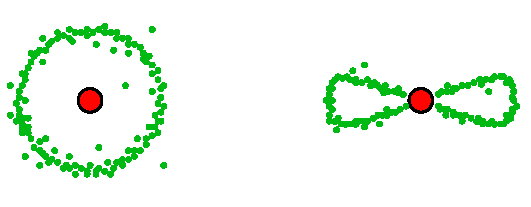
\includegraphics[width=6cm]{figs/electronic_shells/photograph_of_electron.pdf}
    \caption{Пример фиксации положения электрона относительно ядра в различные моменты времени.}
    \label{fig:photograph_of_electron}
\end{figure}

В итоге окажется, что в некоторых областях пространства вокруг ядра электрон бывает чаще всего. Если мы оставим только пространство, в котором мы можем обнаружить электрон, например, в \qty{95}{\percent} случаев, и ограничим это пространство поверхностью, то получим изображение электронного облака. Электронные облака могут быть различной формы. Пример такого облака вы можете увидеть на рис.~\ref{fig:s_and_p_orbitals}.

\begin{figure}[htbp]
    \centering
    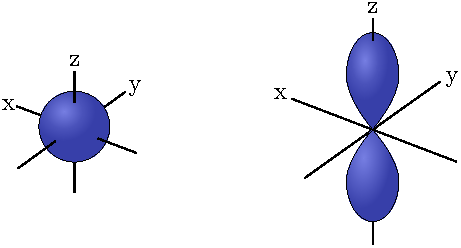
\includegraphics[width=6cm]{figs/electronic_shells/s_and_p_orbitals.pdf}
    \caption{Электронное облако принято изображать поверхностью, в пределах которой электрон пребывает чаще всего.}
    \label{fig:s_and_p_orbitals}
\end{figure}

Второе следствие квантово-механического описания характера движения электрона~--- \emph{дискретность (квантованность)}\label{term:quantization}\index{квантование} параметров. Это означает, что все характеристики электрона не могут меняться непрерывно, а могут принимать только определённые значения.

Например, энергия электрона может принимать только определённые разрешённые значения, и, если электрону нужно перейти в состояние с другой энергией, ему придётся излучить или поглотить электромагнитное излучение с энергией, строго равной разнице между энергетическими уровнями.

Из-за принципа квантования форма электронного облака тоже не может быть какой угодно, а только такой, какую разрешено принимать в соответствии с фундаментальными законами нашего мира.

Принцип квантования необходимо уложить в голове, но со временем вы научитесь мыслить в этом ключе. Давайте рассмотрим, каким именно образом электроны могут распределяться вокруг ядра с точки зрения квантовой теории.

\subsection*{Главное квантовое число}

Энергию электрона в атоме оценивают относительно свободного электрона в вакууме, энергию которого принимают за ноль. Электрону энергетически выгоднее быть связанным с атомным ядром, чем находиться в свободном состоянии, поэтому в атоме потенциальная энергия электрона ниже (имеет более отрицательное значение), чем у свободного.

$e$~--- так обозначают сам электрон и величину его кулоновского заряда\footnote{\qty{-1,602176634e-19}{\C}.}. Поскольку заряд электрона очень мал, энергию электрона выражают обычно в электрон-вольтах (эВ).

Энергия электрона в атоме квантована таким образом: существуют основные уровни, на которых может находиться электрон, которые разделены относительно большими промежутками энергии. Затем эти уровни могут также расщепляться на более мелкие подуровни с относительно небольшой разницей в энергии между ними. (рис.~\ref{fig:energy_levels}).

\begin{figure}[htbp]
    \centering
    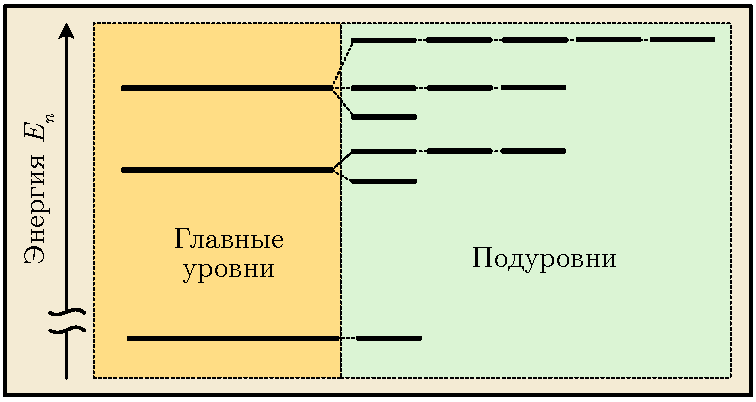
\includegraphics[width=8cm]{figs/electronic_shells/energy_levels.pdf}
    \caption{Значение энергии электрона в атоме может принимать только определённые значения, соответствующие энергетическим уровням.}
    \label{fig:energy_levels}
\end{figure}

Энергия главных уровней пропорциональна величине

\begin{equation}
    E_n \propto -\frac{1}{n^2}.
\end{equation}

где $n$~--- некоторое число, принимающее значения из ряда целых натуральных чисел $n = (1,2,3,4,\ldots,\infty)$.

Число $n$ называют \textbf{главным квантовым числом}\label{term:main_quantum_number}\index{главное квантовое число}. Энергия электронов в атомах (то есть энергия главных уровней) зависит, в основном, именно от этого числа. Чем главное квантовое число больше, тем выше энергия электрона и тем ближе она к энергии свободного электрона в вакууме.

Значения энергии электрона, соответствующие каждому квантовому числу, называют \textbf{энергетическими уровнями}\label{term:energy_level}\index{энергетический уровень}.

Например, если электрон находится на уровне, соответствующему главному квантовому числу $n = 1$, то говорят, что электрон находится на первом энергетическом уровне. Для атома водорода эти уровни показаны на рис.~\ref{fig:energy_levels_of_hydrogen}.

\begin{figure}[htbp]
    \centering
    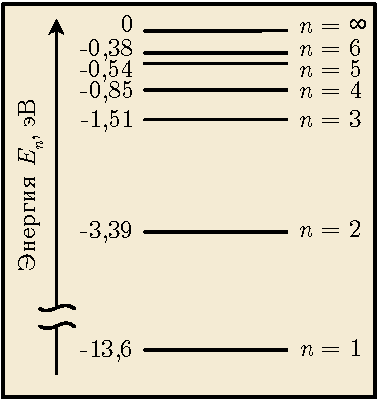
\includegraphics[width=4.6cm]{figs/electronic_shells/energy_levels_of_hydrogen.pdf}
    \caption{Энергетические уровни электрона в атоме водорода.}
    \label{fig:energy_levels_of_hydrogen}
\end{figure}

Обратите внимание на то обстоятельство, что с ростом $n$ разница между энергетическими уровнями быстро уменьшается и при достаточно больших $n$ стремится к нулю, что физически означает отрыв электрона от атома.

Кроме того, из-за такого сближения по энергии уровней со смежными $n$ верхние подуровни более низкого уровня могут оказаться по энергии близки с нижними подуровнями более высокого уровня, из-за чего главные уровни энергии могут быть заполнены электронами не полностью.

Давайте попробуем решить следующую задачу.

\begin{problem}{}{electronic_shells1}
    При переходе электрона между какими уровнями выделится больше энергии: между седьмым и пятым или между пятым и четвёртым?
    \begin{sol}{\ref{prob:electronic_shells1}}
        Энергия электрона пропорциональна
        \begin{equation*}
            E_n \propto -\frac{1}{n^2}
        \end{equation*}
        Следовательно, в первом случае
        \begin{equation*}
            \varDelta E_{7 \rightarrow 5} \propto \frac{1}{5^2} - \frac{1}{7^2} = \frac{1}{25} - \frac{1}{49} \propto \num{0,0196} 
        \end{equation*}
        а во втором
        \begin{equation*}
            \varDelta E_{5 \rightarrow 4} \propto \frac{1}{4^2} - \frac{1}{5^2} = \frac{1}{16} - \frac{1}{25} \propto \num{0,0225} 
        \end{equation*}
        При переходе между пятым и четвёртым уровнем выделится больше энергии.
    \end{sol}
\end{problem}

На каждом энергетическом уровне может располагаться вовсе не произвольное число электронов, а только то, которое разрешено для данного главного квантового числа. Это число равно

\begin{equation}
    \label{eq:number_of_electrons_at_the_main_level}
    \fbox{$N = 2n^2$}.
\end{equation}

Например, на первом энергетическом уровне максимально могут располагаться всего $2 \cdot 1^2 = 2$ электрона, на втором $2 \cdot 2^2 = 8$ и т.~д.

А как располагаются в атоме электроны на энергетических подуровнях в пределах одного уровня? В целом~--- по такому же принципу, занимая только разрешённые состояния. Кроме главного квантового числа $n$ существуют ещё три других квантовых числа, которые как раз описывают состояние электрона в подуровнях:

\begin{itemize}
    \item $l$~--- орбитальное;
    \item $m_l$~--- магнитное;
    \item $m_s$~--- спиновое.
\end{itemize}

Каждое из квантовых чисел характеризует определённое свойство электрона, и при помощи набора \emph{всех четырёх} квантовых чисел можно полностью описать состояние электрона в атоме. Мы постепенно изучим каждое из них.

Обратите внимание вот на что: номер периода, в котором находится химический элемент в периодической таблице, по сути, является главным квантовым числом того энергетического уровня, который является внешним у данного элемента.

Что имеется в виду: каждый последующий химический элемент имеет на один протон в ядре и один электрон на оболочке больше, чем предыдущий. Электроны заполняют электронные оболочки, начиная с самых низких по энергии, то есть сначала заполняется оболочка с главным квантовым числом $n = 1$. На этой оболочке согласно формуле $N = 2n^2$ максимум могут располагаться 2 электрона. Это соответствует всего двум химическим элементам в первом периоде~--- водороду и гелию.

Третий электрон начинает заселять следующую по энергии оболочку с главным квантовым числом $n = 2$. Максимум на ней может разместиться (согласно формуле \ref{eq:number_of_electrons_at_the_main_level}) 8 электронов. Это соответствует восьми химическим элементам от лития до неона во втором периоде. Далее начинает заполняться третий период, четвёртый и так далее.

При этом максимально возможное число электронов на определённом энергетическом уровне не обязательно достигается, например, и во втором, и в третьем периоде по 8 элементов, хотя в третьем их могло бы быть $2 \cdot 3^2 = 18$. Но вместо этого начинает заселяться электронная оболочка с $n = 4$.

Как мы уже упоминали, всё дело в том, что нижние подуровни четвёртой оболочки оказываются ниже по энергии, чем верхние подуровни третьей. Подробнее об этом мы расскажем далее.

Решите следующую задачу. Если не получится, ответ можете посмотреть в \hyperref[sec:solutions]{решениях}.

\begin{problem}{}{electronic_shells2}
    В некоторой параллельной вселенной максимальное число электронов на электронных уровнях равно не $N = 2n^2$, а $N = n^2$. В каком периоде периодической таблицы в этой вселенной будет располагаться углерод?
    \begin{sol}{\ref{prob:electronic_shells2}}
        Углерод находится в периодической таблице под номером 6, следовательно, его атом имеет 6 электронов. На первой электронной оболочке в этой вселенной будет располагаться максимум 1 электрон, на второй~--- 4, на третьей~--- 9. Значит, углерод должен бы иметь на второй оболочке $6 - 1 = 5$ электронов, но там может поместиться только 4. Оставшийся электрон отправится на третий уровень, а углерод окажется в третьем периоде.    
    \end{sol}
\end{problem}

\subsection*{Орбитальное квантовое число}

Как мы уже сказали, графически электронное облако можно представить в виде функции вероятности обнаружить электрон в трёхмерных координатах, ограничивая объём, в котором электрон находится чаще всего с некоторой вероятностью.

То, какой вид будет принимать это облако, определяется \textbf{орбитальным квантовым числом}\label{term:orbital_quantum_number}\index{орбитальное квантовое число} $l$, которое может принимать целые значения от нуля до $(n - 1)$, где $n$~--- это главное квантовое число того энергетического уровня, для которого мы рассчитываем возможные значения $l$.

\begin{equation*}
    \fbox{$l = (0,1,2, \ldots ,n - 1)$}
\end{equation*}

Таким образом, для электрона на первом энергетическом уровне с $n = 1$ орбитальное квантовое число может принимать только одно значение~--- ноль. Для электрона на втором уровне с $n = 2$ орбитальное квантовое число может принимать значения 0 или 1, и т.~д.

Энергия электрона в атоме зависит, в основном, от значения главного квантового числа $n$, однако в атомах, в которых электронов больше одного она зависит также и от орбитального квантового числа. Чем выше квантовое число $l$, тем выше энергия, поэтому состояния электрона, характеризующиеся различными значениями $l$ называют \textbf{энергетическими подуровнями}\label{term:energy_sublevel}\index{энергетический подуровень}.

По историческим причинам для обозначения подуровней используют не сами числовые значения орбитального квантового числа (0, 1, 2), а строчные буквы латинского алфавита\footnote{s, p, d, f –-- первые буквы английских слов <<\textit{sharp}>>~--- резкий, <<\textit{principal}>>~--- главный, <<\textit{diffuse}>>~--- диффузный и <<\textit{fine}>>~--- тонкий. Выглядит странно? Таковы традиции. А вообще~--- так визуально выглядят спектральные линии, соответствующие этим подуровням.} (табл.~\ref{tab:letter_designations_of_energy_sublevels}).

\begin{table}[htbp]
    \small
    \centering
    \caption{Буквенные обозначения энергетических подуровней.}
    \label{tab:letter_designations_of_energy_sublevels}
    \begin{tabular}{cccccc}
        \hline
        \rowcolor{green!5}
        0 & 1 & 2 & 3 & 4 & 5\\
        \hline
        s & p & d & f & g & h\\
        \hline
    \end{tabular}
\end{table}

Чтобы показать, что электрон находится на определённой электронной оболочке, записывают номер энергетического уровня и букву, обозначающую подуровень. Например, s-электроны второго энергетического уровня обозначают 2s, d-электроны третьего уровня~--- 3d.

Как уже было сказано, для первого энергетического уровня в атоме возможно только одно орбитальное квантовое число~--- 0. Поэтому на первом энергетическом уровне могут располагаться только s-электроны, и не может существовать подуровней 1p или 1d.

На втором энергетическом уровне могут находиться только s и p-электроны, но не могут d-электроны, поэтому не существует энергетического уровня 2d (табл.~\ref{tab:available_sublevels}).

\begin{table}[htbp]
    \small
    \centering 
    \caption{Доступные подуровни для энергетических уровней.}
    \label{tab:available_sublevels}
    \begin{tabular}{cccccc}
        \hline
        {\multirow{2}{*}{$n$}} & \multicolumn{5}{c}{$l$} \\ \cline{2-6}
        & 0 & 1 & 2 & 3 & 4 \\ 
        \hline
        5 & s & p & d & f & g \\
        4 & s & p & d & f &   \\
        3 & s & p & d &   &   \\
        2 & s & p &   &   &   \\
        1 & s &   &   &   &   \\
        \hline
    \end{tabular}
\end{table}

Существование соответствующих подуровней вовсе не означает, что на них в атоме обязательно будут находиться электроны. Например, натрий находится в третьем периоде, то есть у него имеется возможность заполнения d-подуровня. Однако электронов всего 11, и до d-подуровня дело не доходит.

\subsection*{Магнитное квантовое число}

Принцип квантования распространяется не только на общую энергию электрона в атоме (главное квантовое число) и форму электронного облака (орбитальное квантовое число), но и на то, как это облако может располагаться в пространстве. Ориентация электронных облаков зависит от \textbf{магнитного квантового числа}\label{term:magnetic_quantum_number}\index{магнитное квантовое число} $m_l$.

Магнитное квантовое число может принимать целые значения от $-l$ до $+l$:

\begin{equation*}
    \fbox{$m_l = (-l, \ldots ,-2,-1,0,1,2, \ldots ,+l)$}.
\end{equation*}

Таким образом, для каждого квантового числа $l$ существует $2l + 1$ возможных значений магнитного квантового числа, то есть возможных ориентаций электронного облака в пространстве.

Например, для s-электронов (для которых орбитальное квантовое число $l = 0$) может существовать $2 \cdot 0 + 1 = 1$ значений магнитного квантового числа ($m_l = 0$), то есть возможна одна-единственная ориентация электронного облака в пространстве. Это связано с тем, что s-электронные облака имеют сферическую симметрию (рис.~\ref{fig:s})

\begin{figure}[htbp]
    \centering
    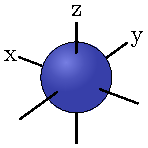
\includegraphics[width=2.5cm]{figs/electronic_shells/s.pdf}
    \caption{s-орбиталь.}
    \label{fig:s}
\end{figure}

В случае p-электронов ($l = 1$) магнитное квантовое число может принимать $2 \cdot 1 + 1 = 3$ различных значения (а именно: $-1$, 0 и 1). Поэтому возможно три различных ориентации p-электронных облаков в пространстве, которые обозначают $\mathrm{p}_x$, $\mathrm{p}_y$ и $\mathrm{p}_z$ (табл.~\ref{tab:p_orbitals}).

\begin{table}[htbp]
    \caption{Возможные ориентации p-орбиталей.}
    \label{tab:p_orbitals}
    \begin{tabularx}{\textwidth}{ZZZ}
        \hline
        \rowcolor{green!5}
        $\mathrm{p}_x$ & $\mathrm{p}_y$ & $\mathrm{p}_z$ \\
        \hline
        \begin{minipage}[c]{3.5cm}
            \adjustbox{margin=5pt}{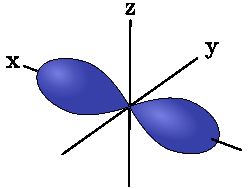
\includegraphics[width=3cm]{figs/electronic_shells/px.pdf}}
        \end{minipage} & 
        \begin{minipage}[c]{3.4cm}
            \adjustbox{margin=5pt}{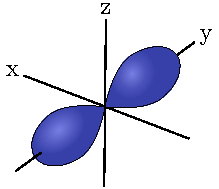
\includegraphics[width=3cm]{figs/electronic_shells/py.pdf}}
        \end{minipage} & 
        \begin{minipage}[c]{3cm}
            \adjustbox{margin=5pt}{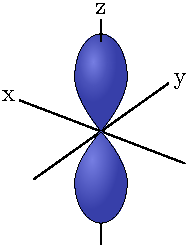
\includegraphics[width=2.5cm]{figs/electronic_shells/pz.pdf}}
        \end{minipage} \\
        \hline
    \end{tabularx}
\end{table}

Оси ($x$, $y$ и $z$), которые показаны на изображениях электронных облаков выбираются произвольно в пространстве и обозначают только положение орбиталей \emph{относительно друг друга и других орбиталей}.

То есть, например, для произвольной p-орбитали мы можем приписать любую из возможных осей, если это не требует определённого контекста (например, отношение к орбиталям соседнего атома или других p-орбиталей).

Для d-электронов количество возможных ориентаций увеличивается ещё на два ($2 \cdot 2 + 1$) и становится равным пяти. Соответствующие ориентации обозначают $\mathrm{d}_{xy}$, $\mathrm{d}_{xz}$, $\mathrm{d}_{yz}$, $\mathrm{d}_{x^2-y^2}$ и $\mathrm{d}_{z^2}$ (табл.~\ref{tab:d_orbitals}).

\begin{table}[htbp]
    \caption{Возможные ориентации d-орбиталей.}
    \label{tab:d_orbitals}
    \begin{tabularx}{\textwidth}{ZZZ}
        \hline
        \rowcolor{green!5}
        $\mathrm{d}_{xy}$ & $\mathrm{d}_{xz}$ & $\mathrm{d}_{yz}$ \\
        \hline
        \begin{minipage}[c]{3.6cm}
            \adjustbox{margin=5pt}{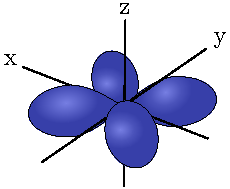
\includegraphics[width=2.8cm]{figs/electronic_shells/dxy.pdf}}
        \end{minipage} & 
        \begin{minipage}[c]{3.6cm}
            \adjustbox{margin=5pt}{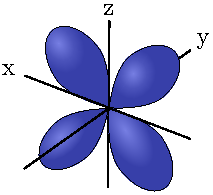
\includegraphics[width=2.8cm]{figs/electronic_shells/dxz.pdf}}
        \end{minipage} & 
        \begin{minipage}[c]{3.6cm}
            \adjustbox{margin=5pt}{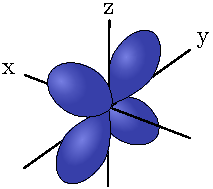
\includegraphics[width=2.8cm]{figs/electronic_shells/dyz.pdf}}
        \end{minipage} \\
        \hline
        \rowcolor{green!5}
        $\mathrm{d}_{x^2-y^2}$ & $\mathrm{d}_{z^2}$ & \\
        \hline
        \begin{minipage}[c]{3.6cm}
            \adjustbox{margin=5pt}{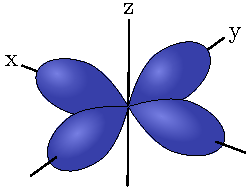
\includegraphics[width=2.8cm]{figs/electronic_shells/dx2-y2.pdf}}
        \end{minipage} & 
        \begin{minipage}[c]{3.2cm}
            \adjustbox{margin=5pt}{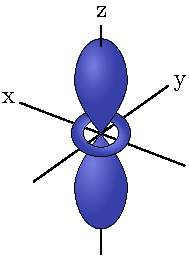
\includegraphics[width=2.2cm]{figs/electronic_shells/dz2.pdf}}
        \end{minipage} & 
        \begin{minipage}[c]{4cm}
        \end{minipage} \\
        \hline
    \end{tabularx}
\end{table}

При помощи набора трёх квантовых чисел, которые мы изучили, можно однозначно охарактеризовать энергию электрона в атоме.

Состояние электрона, которое описывается разрешёнными значениями главного, орбитального и магнитного квантовых чисел, называют \textbf{атомной орбиталью}\label{term:atomic_orbital}\index{атомная орбиталь} (сокращённо АО).

Чтобы показать расположение по энергии, количество и заполнение атомных орбиталей электронами в атоме, орбитали можно представить в виде ячеек, которые располагают в порядке возрастания энергии снизу вверх (рис.~\ref{fig:atomic_orbitals}).

\begin{figure}[htbp]
    \centering
    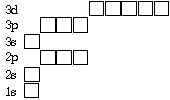
\includegraphics[width=5cm]{figs/electronic_shells/atomic_orbitals.pdf}
    \caption{Изображение атомных орбиталей в виде ячеек.}
    \label{fig:atomic_orbitals}
\end{figure}

Как мы уже упомянули, количество ячеек на каждом энергетическом подуровне равно количеству возможных значений ($2l + 1$) магнитного квантового числа.

\subsection*{Сп\'{и}новое квантовое число. Принцип Паули}

В ходе экспериментов было обнаружено, что каждую атомную орбиталь могут занимать одновременно не более двух электронов. Это привело к открытию ещё одного квантового числа~--- \textbf{спинового}\label{term:spin_quantum_number}\index{спиновое квантовое число} ($m_s$), от английского <<\textit{spin}>>~--- вращение.

Спиновое квантовое число может принимать только одно из двух значений: $+1/2$ или $-1/2$ и показывает разницу между электронами, находящихся на одной атомной орбитали.

Спиновое квантовое число характеризует собственное состояние электрона и не связано с его движением вокруг атомного ядра.

Исторически спиновое квантовое число связывали с вращением электрона вокруг собственной оси, но это не совсем верно. Правильнее рассматривать его как собственную независимую ни от чего характеристику состояния электрона, которая может принимать только два значения.

Для нас самое главное то, является ли спин у рассматриваемых электронов одно- или противоположнонаправленным. Поэтому при составлении диаграмм атомных орбиталей электроны с одним спином обозначают стрелкой вверх $\uparrow $, а с противоположным стрелкой вниз $\downarrow $.

При этом выбор знака спина (или направления стрелки вверх или вниз) является произвольным, важно лишь то, одинаковый он или противоположный (то есть направлены ли стрелки в одну сторону, или в разные).

Например, заполнение атомных орбиталей для атома серы выглядит так, как показано на рис.~\ref{fig:full_atomic_orbitals}.

\begin{figure}[htbp]
    \centering
    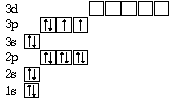
\includegraphics[width=5.5cm]{figs/electronic_shells/full_atomic_orbitals.pdf}
    \caption{Расположение электронов на атомных орбиталях атома серы.}
    \label{fig:full_atomic_orbitals}
\end{figure}

Электроны, находящиеся на одной орбитали и обладающие противоположно направленными спинами, называют \textbf{спаренными}\label{term:paired_electrons}\index{спаренные электроны}. Если на атомной орбитали находится только один электрон, то его называют \textbf{неспаренным}\label{term:unpaired_electrons}\index{неспаренные электроны}.

То, что атомную орбиталь могут занимать не более двух электронов, находит отражение в \textbf{принципе Паули}\label{term:Pauli_principle}\index{принцип Паули}: \emph{в атоме не может быть двух электронов с одинаковым набором всех четырёх квантовых чисел}.

Набор из всех четырёх квантовых чисел \emph{полностью характеризует состояние электрона в атоме}.

Давайте подведём итоги и сведём информацию по всем четырём квантовым числам в табл.~\ref{tab:quantum_numbers}.

\begin{table}[htbp]
    \small
    \caption{Квантовые числа}
    \label{tab:quantum_numbers}
    \begin{tabularx}{\textwidth}{
        >{\hsize=0.8\hsize}Y
        >{\hsize=0.6\hsize}Z
        >{\hsize=1.2\hsize}Z
        >{\hsize=1.4\hsize}Y
        }
        \hline
        \rowcolor{green!5}
        Квантовое число & Обо\-зна\-че\-ние & Какие значения принимает & Что характеризует \\
        \hline
        Главное & $n$ & $1,2,3, \ldots ,\infty$ & Энергию электронного уровня \\
        Орбитальное & $l$ & $0,1,2, \ldots ,n-1$ & Энергию электронного подуровня \\
        Магнитное & $m_l$ & $-l, \ldots ,-1,0,1, \ldots ,+l$ & Ориентацию электронного облака в пространстве \\
        Спиновое & $m_s$ & $+1/2,-1/2$ & Собственное состояние электрона \\
        \hline
    \end{tabularx}
\end{table}

Потренируйтесь в формулировке определений из сегодняшнего урока, в этот раз их довольно много. Затем переходите к решению задач.

\begin{termlist}
    \hyperref[term:Heisenberg_uncertainty_principle]{Принцип неопределённости Гейзенберга}, 
    \hyperref[term:quantization]{квантование}, 
    \hyperref[term:main_quantum_number]{главное квантовое число}, 
    \hyperref[term:energy_level]{энергетический уровень}, 
    \hyperref[term:orbital_quantum_number]{орбитальное квантовое число}, \hyperref[term:energy_sublevel]{энергетический подуровень}, 
    \hyperref[term:magnetic_quantum_number]{магнитное квантовое число}, \hyperref[term:atomic_orbital]{атомная орбиталь}, 
    \hyperref[term:spin_quantum_number]{спиновое квантовое число}, 
    \hyperref[term:paired_electrons]{спаренные электроны}, 
    \hyperref[term:unpaired_electrons]{неспаренные электроны}, 
    \hyperref[term:Pauli_principle]{принцип Паули}.
\end{termlist}

\begin{problem}{}{electronic_shells3}
    Охарактеризуйте квантовыми числами электрон, находящийся на 4s-орбитали. Спиновое квантовое число выберите произвольно. 
    \begin{sol}{\ref{prob:electronic_shells3}}
        4~--- это главное квантовое число данного электрона. s-орбиталь означает, что орбитальное квантовое число равно нулю, то есть $l = 0$ (табл.~\ref{tab:letter_designations_of_energy_sublevels}). Для s-электронов возможно только одно значение магнитного квантового числа~--- 0. Наконец, спиновое квантовое число может принимать любое значение по выбору: $+1/2$ либо $-1/2$, поскольку мы не знаем спин других электронов в этом атоме. Итак, $n = 4, l = 0, m_l = 0, m_s = +1/2$.
    \end{sol}
\end{problem}

\begin{problem}{}{electronic_shells4}
    Какое максимальное число электронов может содержаться на 5d-подуровне? А на 4d-подуровне?
    \begin{sol}{\ref{prob:electronic_shells4}}
        Максимальное число электронов на электронном подуровне не зависит от главного квантового числа и определяется возможным количеством АО, которое равно количеству возможных значений $(2l + 1)$ магнитного квантового числа. На каждой АО может располагаться до двух электронов. d-подуровню соответствует орбитальное квантовое число $l = 2$, поэтому максимальное количество электронов на 5d-подуровне будет равно
        \begin{equation*}
            2(2l + 1) = 2(2 \cdot 2 + 1) = 10.
        \end{equation*}
        На 4d-подуровне также может располагаться 10 электронов.
    \end{sol}
\end{problem}

\begin{problem}{}{electronic_shells5}
    Квантовый сейф открывается комбинацией из трёх чисел $n$, $l$ и $m_l$. Условия такие:
    \begin{itemize}
        \item $n = 2$ или 3;
        \item $l$ допустимо для данного $n$;
        \item $m_l$ допустимо для данного $l$.
    \end{itemize}
    Сколько всего возможных комбинаций? Приведите 5 примеров.
    \begin{sol}{\ref{prob:electronic_shells5}}
        Для $n = 2$:
        \begin{itemize}
            \item $l=0: m_l = 0$~--- 1 вариант;
            \item $l=1: m_l = -1, 0, +1$~--- 3 варианта.
        \end{itemize}
        Итого: $1 + 3 = 4$ комбинации.
        Для $n = 3$:
        \begin{itemize}
            \item $l = 0: m_l = 0$~--- 1 вариант;
            \item $l = 1: m_l = -1, 0, +1$~--- 3 варианта;
            \item $l = 2: m_l = -2, -1, 0, +1, +2$~--- 5 вариантов.
        \end{itemize}
        Итого: $1 + 3 + 5 = 9$ комбинаций.
        Всего: $4 + 9 = 13$ возможных комбинаций.
        Примеры: $(2, 0, 0)$, $(2, 1, -1)$, $(3, 0, 0)$, $(3, 1, +1)$, $(3, 2, -2)$.
    \end{sol}
\end{problem}

\clearpage

\section{Что такое ионы? Электронная конфигурация атомов}

\subsection*{Определение иона}

Теперь мы имеем некоторое представление об электронных оболочках и можем двигаться дальше. В нейтральном атоме количество электронов равно заряду ядра атома, так как атом, в целом, обычно не заряжен. Тем не менее нейтральные атомы в природе встречаются не так уж и часто.

Всё дело в том, что образование химических связей между атомами происходит именно за счёт электронов, а именно~--- выигрыша в энергии из-за изменения их энергетического состояния.

Изменения состояния электронов представляют собой переходы между энергетическими уровнями орбиталей атома или образовавшейся системы атомов, поэтому то, как происходит заполнение электронных оболочек очень важно для дальнейшего понимания концепции химической связи.

Итак, к атому химического элемента можно добавить или отнять электроны. Это можно сделать, потому что у любого атома имеются как занятые, так и пустые атомные орбитали. При этом атомам энергетически наиболее выгодны два варианта обмена своими электронами:

\begin{itemize}
    \item принять электроны на пустые орбитали с наименьшей энергией (то есть орбитали с наименьшими значениями $n$ и $l$). Их называют \textbf{нижние свободные атомные орбитали}\label{term:lower_empty_atomic_orbital}\index{НСАО} (НСАО);
    \item отдать электроны с \textbf{верхних занятых атомных орбиталей}\label{term:upper_filled_atomic_orbital}\index{ВЗАО} (ВЗАО).
\end{itemize}

Например, для атома бора нижними свободными орбиталями являются две пустые 2p-орбитали, а верхней занятой является 2p-орбиталь, на которой имеется один электрон (рис.~\ref{fig:boundary_orbitals}).

При этом в химических реакциях атом не может присоединить или отдать сколько угодно электронов. Запомните: атом принимает и отдаёт электроны только в пределах того энергетического уровня, который у него является внешним.

Для бора внешним является энергетический уровень с главным квантовым числом $n = 2$, на котором может помещаться до восьми электронов. Поэтому атом бора может присоединить до пяти или отдать до трёх электронов.

\begin{figure}[htbp]
    \centering
    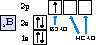
\includegraphics[width=4.5cm]{figs/electronic_configuration/boundary_orbitals.pdf}
    \caption{ВЗАО и НСАО в атоме бора.}
    \label{fig:boundary_orbitals}
\end{figure}

Почему так происходит? Возможность того, что атом удержит электроны возле себя, определяется балансом двух факторов:

\begin{itemize}
    \item притяжением положительно заряженного ядра и электронов (при этом чем дальше находятся электроны от ядра, тем слабее это взаимодействие);
    \item взаимным отталкиванием и эффектом экранирования электронов друг друга\footnote{Имеется в виду то, что внутренние электронные оболочки снижают энергию взаимодействия атомного ядра и внешних электронных оболочек.}.
\end{itemize}

Заряд ядра атома и его способность удерживать электроны растут с увеличением зарядового числа $Z$. Если к атому с небольшим зарядом (например, азоту) добавить электроны, которые вынуждены будут располагаться на орбиталях с $n = 3$, то они окажутся довольно далеко от ядра, а также будут экранированы электронами, находящимися на более низких уровнях. Такая электронная конфигурация будет невыгодна для ядра с таким зарядовым числом.

Однако если количество протонов в ядре будет больше (как в более тяжёлых химических элементах), то такое ядро уже сможет удерживать возле себя большее количество электронов, что мы и наблюдаем в последующих химических элементах.

Обратите внимание вот на что: каждый период в периодической таблице заканчивается элементом, в котором внешняя электронная оболочка полностью заполнена. Это гелий, неон, аргон, криптон, ксенон и радон.

Электронные оболочки у этих элементов настолько устойчивы, что они не склонны вступать в какие бы то ни было химические реакции (точнее, вступают, но с большим трудом). Эти элементы называют \textbf{благородными газами}\label{term:noble_gases}\index{благородные газы}.

Итак, если к атому присоединить или отдать ему электроны, то он перестанет быть электронейтральным и приобретёт заряд, поскольку количество протонов в ядре не будет равно количеству электронов. В этом случае атом станет ионом.

\textbf{Ион}\label{term:ion}\index{ион}~--- это заряженная частица, которая образуется в результате отдачи или присоединения электронов.

Почему мы говорим о частице, а не только об атоме? Ионы могут быть \emph{простыми} (например, хлорид-ион \ce{Cl^-}) и \emph{сложными} (многоатомными, например, сульфат-ион \ce{SO_4^2-}), потому что в химических соединениях положительный или отрицательный заряд может располагаться как на отдельном атоме, так и быть <<размазанным>> по всей молекуле, в этом случае заряд приписывают всей частице.

Положительно заряженные ионы называют \textbf{катионами}\label{term:cation}\index{катион}. Они содержат меньше электронов, чем нейтральный атом.

Отрицательно заряженные ионы называют \textbf{анионами}\label{term:anion}\index{анион}. Они содержат больше электронов, чем нейтральный атом.

Заряд иона записывают сверху справа после символа атома или группы атомов. При этом сначала указывают величину заряда (если она больше единицы), а затем знак заряда. Вот несколько примеров катионов:

\begin{itemize}
    \item \ce{H^+} катион водорода (читается «аш плюс»),
    \item \ce{Ca^2+} катион кальция (читается «кальций два плюс»),
    \item \ce{NH_4^+} катион аммония (читается «эн аш четыре плюс»).
\end{itemize}

И анионов:

\begin{itemize}
    \item \ce{S^2-} сульфид-анион (читается «эс два минус»),
    \item \ce{Cl^-} хлорид-анион (читается «хлор минус»),
    \item \ce{CO_3^2-} карбонат-анион (читается «це о три два минус»).
\end{itemize}

Теперь покажем, какими способами можно указать распределение электронов по уровням в атомах, если вам необходимо записать или передать эту информацию.

В зависимости от того, на каких именно особенностях распределения вы хотите сделать акцент, можно использовать три основных способа записи электронной конфигурации.

\subsection*{Электроны на энергетических уровнях (только главное квантовое число)}

Если необходимо показать только главные электронные уровни в атоме и общее число электронов на них, можно использовать схему наподобие той, что показана на рис.~\ref{fig:electronic_levels_Al}.

\begin{figure}[htbp]
    \centering
    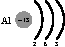
\includegraphics[width=3cm]{figs/electronic_configuration/Al.pdf}
    \caption{Заполнение энергетических уровней атома алюминия.}
    \label{fig:electronic_levels_Al}
\end{figure}

В этом случае необходимо сначала записать символ атома и заряд его ядра, а затем в виде дуг обозначить электронные оболочки атома и снизу указать количество электронов на них.

Каждая электронная оболочка подразумевает, что все электроны, находящиеся на ней, обладают одинаковым значением главного квантового числа $n$.

Такая запись удобна, если необходимо показать электронную конфигурацию иона (рис.~\ref{fig:electronic_levels_Al3+}). В этом случае хорошо видно увеличение или уменьшение числа электронов на внешней электронной оболочке атома. Обратите внимание на устойчивую восьмиэлектронную конфигурацию катиона алюминия.

\begin{figure}[htbp]
    \centering
    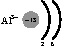
\includegraphics[width=2.8cm]{figs/electronic_configuration/Al3+.pdf}
    \caption{Заполнение энергетических уровней катиона алюминия.}
    \label{fig:electronic_levels_Al3+}
\end{figure}

При образовании иона \ce{Al^3+} атом теряет три электрона со внешней электронной оболочки с главным квантовым числом $n = 3$ и остаётся с двумя полностью заполненными электронными оболочками.

Положительно заряженные ионы имеют на электронных оболочках меньшее число электронов, чем соответствующий нейтральный атом. В отрицательно заряженных ионах, наоборот, происходит увеличение числа электронов на оболочках.

Например, в бромид-ионе \ce{Br^-} на один электрон больше на внешней электронной оболочке, чем у нейтрального атома (рис.~\ref{fig:electronic_levels_Br}). И снова~--- восьмиэлектронная конфигурация.

\begin{figure}[htbp]
    \centering
    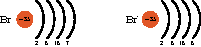
\includegraphics[width=9cm]{figs/electronic_configuration/Br_Br-.pdf}
    \caption{Заполнение энергетических уровней атома брома и аниона брома.}
    \label{fig:electronic_levels_Br}
\end{figure}

В ионе \ce{Br^+} наоборот, на один электрон меньше (рис.~\ref{fig:electronic_levels_Br+}).

\begin{figure}[htbp]
    \centering
    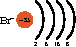
\includegraphics[width=3.4cm]{figs/electronic_configuration/Br+.pdf}
    \caption{Энергетические уровни катиона брома.}
    \label{fig:electronic_levels_Br+}
\end{figure}

\subsection*{Энергетические уровни и подуровни (главное и орбитальное квантовые числа)}

Если вам нужно показать распределение электронов более подробно, скажем, не только по энергетическим уровням (главное квантовое число $n$), но и по подоболочкам (орбитальное квантовое число $l$), то используют вот такую строчную запись:

\begin{equation*}
    \ce{Na{:}}\ 1\mathrm{s}^22\mathrm{s}^22\mathrm{p}^63\mathrm{s}^1.
\end{equation*}

При этом цифрой указывают номер электронной оболочки (главное квантовое число), затем буквенное обозначение орбитального квантового числа (s, p, d, f \ldots) и над ним верхним индексом число электронов на соответствующем подуровне (рис.~\ref{fig:electronic_notation}).

\begin{figure}[htbp]
    \centering
    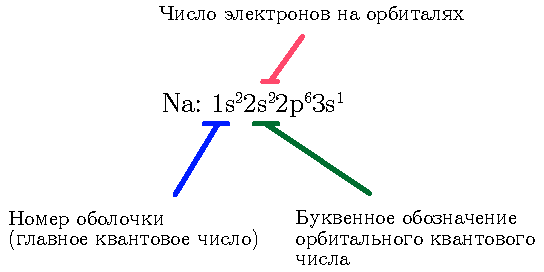
\includegraphics[width=8cm]{figs/electronic_configuration/electronic_notation.pdf}
    \caption{Строчная запись электронной конфигурации.}
    \label{fig:electronic_notation}
\end{figure}

Например, для атома серы электронная конфигурация будет следующей:

\begin{equation*}
    \ce{S{:}}\ 1\mathrm{s}^22\mathrm{s}^22\mathrm{p}^63\mathrm{s}^23\mathrm{p}^4.
\end{equation*}

Впрочем, для экономии места чаще используют сокращённую запись электронной конфигурации, указывая только конфигурацию внешней электронной оболочки. При этом подразумевается, что все нижележащие оболочки полностью заполнены:

\begin{equation*}
    \ce{S{:}}\ 3\mathrm{s}^23\mathrm{p}^4
\end{equation*}

Если всегда использовать только полную запись, ваша продуктивность сильно пострадает. Попробуйте записать полную электронную конфигурацию для атома какого-нибудь висмута.

Иногда, чтобы показать факт полного заполнения электронных подоболочек, в квадратных скобках перед электронной конфигурацией указывают символ ближайшего благородного газа:

\begin{equation*}
    \ce{S{:}}\ [\ce{Ne}]3\mathrm{s}^23\mathrm{p}^4.
\end{equation*}

В периодической таблице электронную конфигурацию, записанную одной из таких строчных записей, обычно указывают непосредственно в ячейке химического элемента, как показано на рис.~\ref{fig:electronic_configuration_in_periodic_table}.

\begin{figure}[htbp]
    \centering
    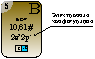
\includegraphics[width=5.5cm]{figs/electronic_configuration/electronic_configuration_in_periodic_table.pdf}
    \caption{Электронная конфигурация в ячейках периодической таблицы.}
    \label{fig:electronic_configuration_in_periodic_table}
\end{figure}

Поскольку каждую атомную орбиталь могут занимать не более двух электронов, то максимальное число электронов на энергетическом подуровне с орбитальным квантовым числом $l$ равно $2(2l + 1)$ (табл.~\ref{tab:maximum_capacity_of_energy_sublevels}). На сегодняшний день в периодической системе химических элементов нет элементов с электронами на подуровнях выше f.

\begin{table}[htbp]
    \centering
    \caption{Максимальная ёмкость энергетических подуровней.}
    \label{tab:maximum_capacity_of_energy_sublevels}
    \begin{tabular}{ccc}
        \hline
        \rowcolor{green!5}
        Энергетический подуровень & $l$ & Максимально возможное число электронов \\
        \hline
        s & 0 & 2 \\
        p & 1 & 6 \\
        d & 2 & 10 \\
        f & 3 & 14 \\
        \hline
    \end{tabular}
\end{table}

\subsection*{Электронные оболочки, подоболочки и распределение по атомным орбиталям}

В самом подробном типе записи вы должны полностью показать распределение электронов в атоме. Необходимо указать по каким орбиталям распределены электроны и какой спин они имеют.

Для этого следует нарисовать уже знакомую вам диаграмму с ячейками, которые соответствуют отдельным атомным орбиталям, как это показано на рис.~\ref{fig:S_electronic_configuration_AO}.

\begin{figure}[htbp]
    \centering
    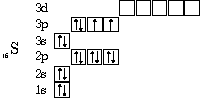
\includegraphics[width=6cm]{figs/electronic_configuration/S_electronic_configuration.pdf}
    \caption{Электронная конфигурация атома серы в виде ячеек АО.}
    \label{fig:S_electronic_configuration_AO}
\end{figure}

На таких диаграммах хорошо видно, насколько заполнены электронные оболочки и количество неспаренных электронов. Кстати, вы задумались, а как определить, какое количество электронов должно быть неспаренным?

В атоме серы может существовать и альтернативная конфигурация, когда на 3p-оболочке четыре электрона занимают две атомные орбитали, а третья остаётся свободной. Какой вариант верный~--- узнаем в разделе~\ref{sec:rules_for_filling_electronic_shells}.

\begin{termlist}
    \hyperref[term:lower_empty_atomic_orbital]{НСАО}, 
    \hyperref[term:upper_filled_atomic_orbital]{ВЗАО},
    \hyperref[term:noble_gases]{благородные газы}, 
    \hyperref[term:ion]{ион}, 
    \hyperref[term:cation]{катион}, 
    \hyperref[term:anion]{анион}.
\end{termlist}

\begin{problem}{}{electronic_configuration1}
    Бериллий имеет электронную конфигурацию $1\mathrm{s}^22\mathrm{s}^2$. Какие орбитали являются его ВЗАО и НСАО?
    \begin{sol}{\ref{prob:electronic_configuration1}}
        ВЗАО~--- 2s, НСАО~--- 2p.
    \end{sol}
\end{problem}

\begin{problem}{}{electronic_configuration2}
    Азот имеет электронную конфигурацию $1\mathrm{s}^22\mathrm{s}^22\mathrm{p}^3$. Какие ионы теоретически могут образовываться из атома азота?
    \begin{sol}{\ref{prob:electronic_configuration2}}
        Атом азота может достраивать свою электронную оболочку до октета, принимая электроны на 2p-орбитали. В этом случае образуются ионы \ce{N^-}, \ce{N^2-} и \ce{N^3-}. Также атом азота может отдать электроны с внешней электронной оболочки, пока она не опустошится. В этом случае возможны ионы \ce{N^+}, \ce{N^2+}, \ce{N^3+}, \ce{N^4+} и \ce{N^5+}. Отметим, что теоретическая возможность заполнять или опустошать внешнюю электронную оболочку не означает, что такие ионы будут образовываться на практике. 
    \end{sol}
\end{problem}

\begin{problem}{}{electronic_configuration3}
    Напишите электронную конфигурацию иона \ce{S^2-}.
    \begin{sol}{\ref{prob:electronic_configuration3}}
        Электронная конфигурация нейтрального атома серы~--- $1\mathrm{s}^22\mathrm{s}^22\mathrm{p}^63\mathrm{s}^23\mathrm{p}^4$. Ион \ce{S^2-} имеет на электронной оболочке два дополнительных электрона, которые продолжат заполнение 3p-подуровня. Электронная конфигурация иона будет $1\mathrm{s}^22\mathrm{s}^22\mathrm{p}^63\mathrm{s}^23\mathrm{p}^6$.
    \end{sol}
\end{problem}

\begin{problem}{}{electronic_configuration4}
    Некоторая частица имеет электронную конфигурацию $1\mathrm{s}^22\mathrm{s}^22\mathrm{p}^63\mathrm{s}^23\mathrm{p}^6$.
    \begin{itemize}
        \item Может ли это быть нейтральный атом? Если да~--- какого элемента?
        \item Если это ион, какие варианты возможны? Приведите минимум 3 примера.
    \end{itemize}
    \begin{sol}{\ref{prob:electronic_configuration4}}
        Сумма электронов будет равна $2 + 2 + 6 + 2 + 6 = 18$. Элемент с 18 электронами~--- аргон. Конфигурация соответствует октету (уровень с $n = 3$ заполнен). Возможные варианты ионов: \ce{K^+}, \ce{Ca^2+}, \ce{Cl^-} и \ce{S^2-}.
    \end{sol}
\end{problem}

\begin{problem}{}{electronic_configuration5}
    Ионы \ce{K^+} и \ce{Cl^-} имеют одинаковую электронную конфигурацию ([\ce{Ar}]).
    \begin{itemize}
        \item Почему их радиусы различаются?
        \item Какой ион больше по размеру? Почему?
    \end{itemize}
    \begin{sol}{\ref{prob:electronic_configuration5}}
        У \ce{K^+} больше заряд ядра при той же электронной конфигурации, поэтому у него сильнее притяжение электронов к ядру. Из-за этого радиус катиона калия меньше, а аниона хлора больше.
    \end{sol}
\end{problem}

\begin{problem}{}{electronic_configuration6}
    Может ли существовать ион \ce{O^3-}? Почему?
    \begin{sol}{\ref{prob:electronic_configuration6}}
        Не может. Для этого пришлось бы добавить 3 электрона, два из которых заполнят уровень с $n = 2$, а третий кислороду пришлось бы размещать на уровне с $n = 3$, который имеет высокую энергию.
    \end{sol}
\end{problem}

\clearpage

\section{Правила заполнения электронных оболочек}\label{sec:rules_for_filling_electronic_shells}

\begin{wrapfigure}{r}{0.4\textwidth}
    \centering
    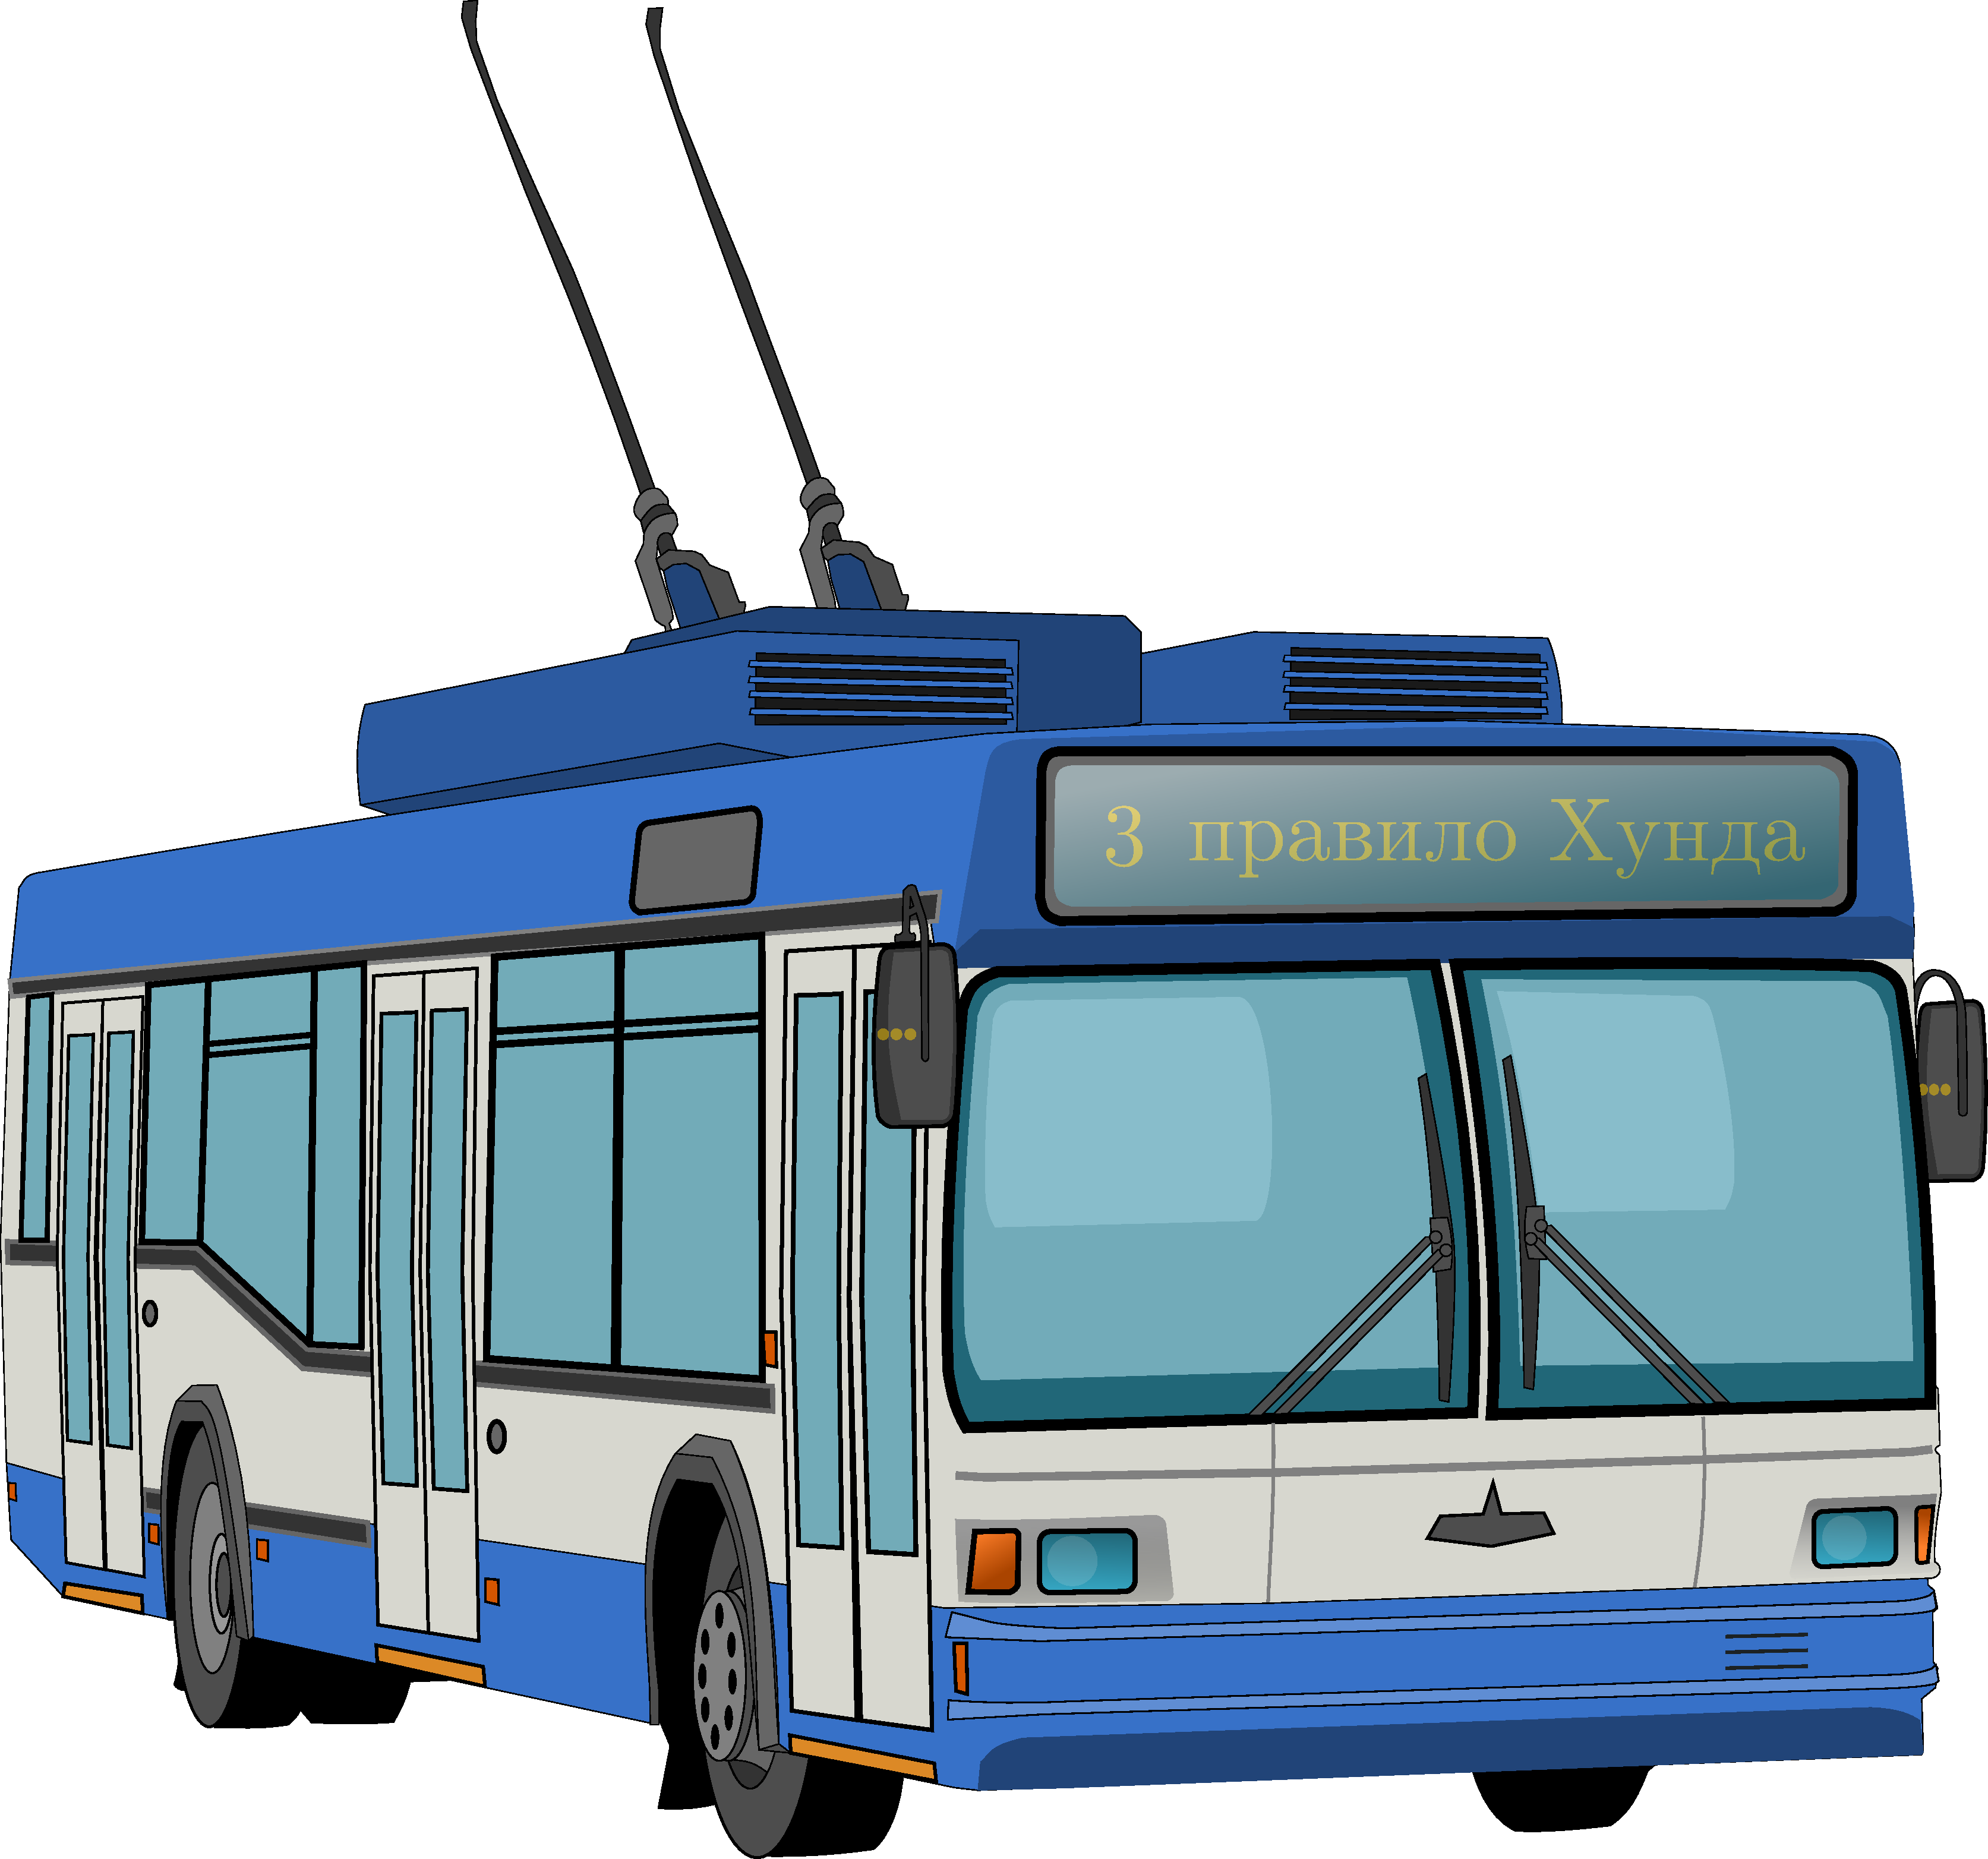
\includegraphics[width=5cm]{figs/rules_for_filling_electronic_shells/trolleybus.pdf}
\end{wrapfigure}

\hspace*{\parindent}Как вы уже поняли, электроны на оболочках предпочитают определённые конфигурации в большей степени, чем другие. Разумеется, это связано с принципом минимальной энергии.

Энергия электрона в атоме определяется значением как главного, так и орбитального квантовых чисел. Это связано с тем, что имеющие более высокую энергию электроны экранируются нижележащими электронами. Поэтому электронные уровни в атоме заполняются в порядке возрастания энергии согласно определённым правилам.

К счастью, для того, чтобы понять эти правила нет необходимости рассчитывать какие-то показатели по сложным формулам, эти правила довольно просты. Давайте их рассмотрим.

\subsection*{Первое правило Клечковского}

Согласно \textbf{первому правилу Клечковского}\label{term:Klechkovsky_first_rule}\index{первое правило Клечковского}, заполнение электронных уровней в атоме происходит в порядке возрастания суммы $n + l$.

Например, ответим на вопрос, какой электронный подуровень заполняется раньше~--- 3d или 4s? Для 3d подуровня сумма $n + l$ равна $(3 + 2) = 5$, а для 4s она равна $(4 + 0) = 4$. Поэтому подуровень 4s заполняется раньше, чем 3d.

\subsection*{Второе правило Клечковского}

Согласно \textbf{второму правилу Клечковского}\label{term:Klechkovsky_second_rule}\index{второе правило Клечковского}, если сумма $n + l$ окажется одинаковой, то первым происходит заполнение электронного подуровня, имеющего меньшее значение $n$.

Например, какой подуровень будет заполняться раньше~--- 3p или 4s? У обоих подуровней сумма $n + l = 4$, однако у 3p подуровня $n = 3$, а у 4s $n = 4$, поэтому первым будет заполняться подуровень 3p.

Пользуясь обоими правилами Клечковского, можно составить общий ряд заполнения электронных оболочек в атоме:
\begin{equation*}
    \label{eq:sequence_of_filling_electronic_subshells}
    \begin{split}
        1s < 2s < 2p < 3s < 3p < 4s < 3d < 4p < 5s < 4d < \\ 
        < 5p < 6s < 4f \sim 5d < 6p < 7s < 5f \sim 6d < 7p.
    \end{split}
\end{equation*}
Подуровни 4f и 5d, а также 5f и 6d очень близки по энергиям.

\subsection*{Правило Хунда}\label{term:hund_rule}\index{правило Хунда}

Иногда имя этого учёного (нем. \textit{Friedrich Hund}) записывают как <<Гунд>>. Также его называют <<правилом троллейбуса>>. Звучит оно следующим образом: при размещении электронов по атомным орбиталям в пределах одной электронной подоболочки электроны располагаются таким образом, чтобы их суммарный спин был максимален.

Проиллюстрируем правило Хунда на примере заполнения 2p-оболочки атома азота. На 2p уровне азота располагаются 3 электрона, которые можно разместить по атомным орбиталям различными способами.

В первом случае (рис.~\ref{fig:N_electronic_configuration_1_var}) суммарный спин электронов равен

\begin{equation*}
    \frac{1}{2} - \frac{1}{2} + \frac{1}{2} = \frac{1}{2}.
\end{equation*}

\begin{figure}[htbp]
    \centering
    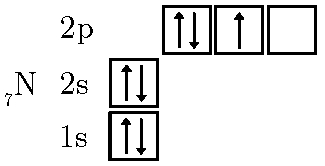
\includegraphics[width=3.5cm]{figs/rules_for_filling_electronic_shells/N_electronic_configuration_1_var.pdf}
    \caption{Первый способ размещения электронов на орбиталях атома азота.}
    \label{fig:N_electronic_configuration_1_var}
\end{figure}

Во втором случае (рис.~\ref{fig:N_electronic_configuration_2_var}):

\begin{equation*}
    \frac{1}{2} + \frac{1}{2} + \frac{1}{2} = \frac{3}{2}.
\end{equation*}

\begin{figure}[htbp]
    \centering
    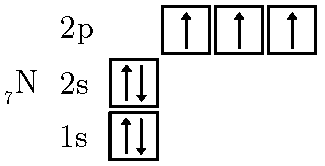
\includegraphics[width=3.5cm]{figs/rules_for_filling_electronic_shells/N_electronic_configuration_2_var.pdf}
    \caption{Второй способ размещения электронов на орбиталях атома азота.}
    \label{fig:N_electronic_configuration_2_var}
\end{figure}

И в третьем случае (рис.~\ref{fig:N_electronic_configuration_3_var}):

\begin{equation*}
    \frac{1}{2} + \frac{1}{2} - \frac{1}{2} = \frac{1}{2}
\end{equation*}

\begin{figure}[htbp]
    \centering
    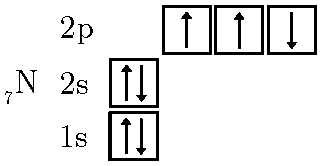
\includegraphics[width=3.5cm]{figs/rules_for_filling_electronic_shells/N_electronic_configuration_3_var.pdf}
    \caption{Третий способ размещения электронов на орбиталях атома азота.}
    \label{fig:N_electronic_configuration_3_var}
\end{figure}

Наибольшим суммарным спином обладает второй способ размещения электронов, поэтому будет реализован именно он. Это вовсе не означает, что другие способы размещения электронов (например, первый и третий) невозможны. Это означает, что способ размещения электронов, удовлетворяющий правилу Хунда, является \emph{основным} и имеет минимальную энергию. Все остальные варианты размещения электронов являются \emph{возбуждёнными}.

Вы догадались, почему это правило называют <<правилом троллейбуса>>? Представьте пустой троллейбус, в который садятся и рассаживаются по сиденьям незнакомые люди. Первым делом они будут занимать все полностью свободные сиденья и только после того, как свободных сидений не останется, они начнут подсаживаться вторым пассажиром на сиденья с людьми.

Однако не все химические элементы следуют вышеописанным правилам, и сейчас мы разберём некоторые примеры.

\subsection*{Исключения из правил Клечковского}

В ряде химических элементов заполнение электронных оболочек происходит с нарушением правил Клечковского. Например, рассмотрим два смежных химических элемента в периодической таблице: никель и медь. У никеля на электронных оболочках содержится 28 электронов, а у меди~--- 29. У никеля в полном соответствии с правилами Клечковского, сначала происходит заполнение 4s подуровня, а только затем 3d, поэтому никель относится к d-элементам (рис.~\ref{fig:Ni_electronic_configuration}).

\begin{figure}[htbp]
    \centering
    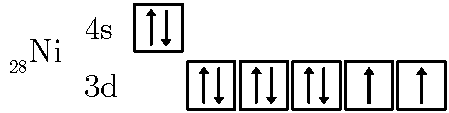
\includegraphics[width=4.7cm]{figs/rules_for_filling_electronic_shells/Ni_electronic_configuration.pdf}
    \caption{Электронная конфигурация атома никеля.}
    \label{fig:Ni_electronic_configuration}
\end{figure}

Медь, имеющая на один электрон больше, в принципе, должна иметь электронную конфигурацию $[\ce{Ar}]3\mathrm{d}^94\mathrm{s}^2$, однако вместо этого один из электронов 4s-подуровня переходит на уровень 3d, в результате чего медь имеет электронную конфигурацию $[\ce{Ar}]3\mathrm{d}^{10}4\mathrm{s}^1$ (рис.~\ref{fig:Cu_electronic_configuration}).

\begin{figure}[htbp]
    \centering
    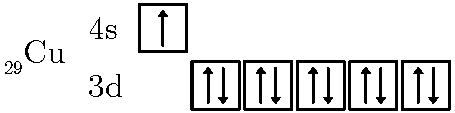
\includegraphics[width=4.7cm]{figs/rules_for_filling_electronic_shells/Cu_electronic_configuration.pdf}
    \caption{Электронная конфигурация атома меди.}
    \label{fig:Cu_electronic_configuration}
\end{figure}

Такое явление называется \textbf{провалом} или \textbf{проскоком}\label{term:electron_slip}\index{проскок электрона} электрона. Причина его в том, что полностью или ровно наполовину заполненные электронные оболочки обладают дополнительной устойчивостью и становится выгоднее завершить 3d оболочку, а не оставлять на ней 9 электронов.

Термин <<провал>> электрона всё же не совсем удачный, потому что принцип минимума энергии для орбиталей всё равно соблюдается: 4s орбиталь у большинства атомов имеет более низкую энергию, чем 3d. Поэтому лучше использовать термин <<проскок>> электрона.

Кроме меди, проскок электрона наблюдается также у хрома, серебра, золота, палладия, ниобия, молибдена, рутения и платины.

В целом нет необходимости каждый раз проводить расчёт и оценивать устойчивость той или иной электронной конфигурации для химических элементов, поскольку строение внешней электронной оболочки атомов вы всегда сможете посмотреть в расширенных версиях \hyperref[appendix:periodic_table]{периодической таблицы}.

\subsection*{Устойчивые электронные конфигурации}

Итак, как вы уже сами убедились, атомы в целом тяготеют к некоторым электронным конфигурациям в большей степени, чем к другим. На это есть, по крайней мере, три причины:

\begin{enumerate}[label=\arabic*)]
    \item \textit{Минимальная энергия}: заполненные/полузаполненные подуровни имеют наименьшую возможную энергию в рамках квантово‑механических правил.
    \item \textit{Симметрия}: равномерное распределение электронов снижает электростатическое отталкивание.
    \item \textit{Квантовые эффекты}: для d-элементов важны обменные взаимодействия и спин‑орбитальное взаимодействие, в суть которых мы не будем вдаваться в рамках нашего обучения.
\end{enumerate}

Поэтому чаще всего в атомах и ионах мы наблюдаем следующие конфигурации:

\begin{itemize}
    \item \textit{Полностью заполненные внешние s- и p-подуровни} (октет: $\mathrm{s}^2\mathrm{p}^6$, то есть 8 электронов), либо заполненный 1s-подуровень (дублет: $1\mathrm{s}^2$, то есть 2 электрона). Это, например, благородные газы:
    \begin{itemize}
        \item \ce{He}: $1\mathrm{s}^2$;
        \item \ce{Ne}: $1\mathrm{s}^22\mathrm{s}^22\mathrm{p}^6$.
    \end{itemize}
    Их химическая инертность~--- прямое следствие этой устойчивости. Ионы также часто стремятся к октету:
    \begin{itemize}
        \item \ce{Na^+}: $1\mathrm{s}^22\mathrm{s}^22\mathrm{p}^6$ (как \ce{Ne});
        \item \ce{Cl^-}: $1\mathrm{s}^22\mathrm{s}^22\mathrm{p}^{6}3\mathrm{s}^23\mathrm{p}^6$ (как \ce{Ar}).
    \end{itemize}
    \item \textit{Полузаполненные d-орбитали}. Для d-элементов (переходные металлы) особенно стабильны конфигурации с полузаполненным d-подуровнем ($\mathrm{d}^5$). Это связано с симметрией распределения электронов. Примеры:
    \begin{itemize}
        \item Mn: [\ce{Ar}]$3\mathrm{d}^54\mathrm{s}^2$;
        \item Re: [\ce{Xe}]$4\mathrm{f}^{14}5\mathrm{d}^56\mathrm{s}^2$.
    \end{itemize}
    \item \textit{Полностью заполненные d-орбитали}. Конфигурация с полностью заполненным d-подуровнем ($\mathrm{d}^{10}$) также высокоустойчива:
    \begin{itemize}
        \item \ce{Zn}: [\ce{Ar}]$3\mathrm{d}^{10}4\mathrm{s}^2$;
        \item \ce{Hg}: [\ce{Xe}]$4\mathrm{f}^{14}5\mathrm{d}^{10}6\mathrm{s}^2$.
    \end{itemize}
    \item \textit{<<Проскок>> электрона} (аномальное заполнение d-орбитали). Некоторые элементы стабилизируют конфигурацию за счёт перехода электрона с $n$s- на $(n - 1)$d-подуровень:
    \begin{itemize}
        \item \ce{Cr}: [\ce{Ar}]$3\mathrm{d}^54\mathrm{s}^1$ (вместо $3\mathrm{d}^44\mathrm{s}^2$);
        \item \ce{Cu}: [\ce{Ar}]$3\mathrm{d}^{10}4\mathrm{s}^1$ (вместо $3\mathrm{d}^94\mathrm{s}^2$).
    \end{itemize}
    Это снижает энергию системы благодаря симметрии d-подуровня.
\end{itemize}

Сможете сформулировать новые понятия? В этот раз их немного.

\begin{termlist}
    \hyperref[term:Klechkovsky_first_rule]{Первое правило Клечковского}, 
    \hyperref[term:Klechkovsky_second_rule]{второе правило Клечковского}, 
    \hyperref[term:hund_rule]{правило Хунда}, 
    \hyperref[term:electron_slip]{проскок электрона}.
\end{termlist}

\begin{example}{}{ex:rules_for_filling_electronic_shells1}
    \textit{Некоторый химический элемент имеет два электрона на 3d-подуровне. Напишите его электронную конфигурацию и выясните, что это за элемент?}

    \medskip

    \textit{Решение.} Согласно \hyperref[eq:sequence_of_filling_electronic_subshells]{последовательности заполнения} электронных подоболочек у элемента с внешними электронами на 3d-подуровне перед ним должны заселяться подуровни 1s, 2s, 2p, 3s, 3p и 4s. Поэтому электронная конфигурация искомого элемента будет $1\mathrm{s}^22\mathrm{s}^22\mathrm{p}^{6}3\mathrm{s}^23\mathrm{p}^64\mathrm{s}^23\mathrm{d}^2$.

    \medskip

    Общее число электронов у элемента будет равно $2 + 2 + 6 + 2 + 6 + 2 + 2 = 22$. Число электронов нейтрального атома равно зарядовому числу $Z$ ядра атома и порядковому номеру элемента в \hyperref[appendix:periodic_table]{периодической таблице}. Это элемент титан.
\end{example}

\begin{example}{}{ex:rules_for_filling_electronic_shells2}
    \textit{Химические элементы имеют на электронных оболочках 28 и 54 электрона. В каких периодах они находятся?}

    \medskip

    \textit{Решение.} Период, в котором находится химический элемент, определяется максимальным главным квантовым числом оболочек, содержащих электроны. При этом не имеет значения, какое $n$ будет у внешней незаполненной подоболочки. Например, элемент титан из примера выше имеет внешние электроны на 3d-подоболочке, однако находится в четвёртом периоде, так как перед этим у него происходит заселение 4s-подуровня.

    \medskip

    Размещаем электроны по подуровням в порядке возрастания суммы $n + l$, пока не будет размещено 28 и 54 электрона. Электронная конфигурация первого элемента: $1\mathrm{s}^22\mathrm{s}^22\mathrm{p}^{6}3\mathrm{s}^23\mathrm{p}^64\mathrm{s}^23\mathrm{d}^8$~--- это никель, четвёртый период. Для второго~--- $1\mathrm{s}^22\mathrm{s}^22\mathrm{p}^{6}3\mathrm{s}^23\mathrm{p}^64\mathrm{s}^23\mathrm{d}^{10}4\mathrm{p}^65\mathrm{s}^24\mathrm{d}^{10}5\mathrm{p}^6$, это ксенон, пятый период.
\end{example}

\begin{problem}{}{rules_for_filling_electronic_shells1}
    Напишите электронную конфигурацию атома фосфора.
    \begin{sol}{\ref{prob:rules_for_filling_electronic_shells1}}
        $[\ce{Ne}]3\mathrm{s}^23\mathrm{p}^3$.
    \end{sol}
\end{problem}

\begin{problem}{}{rules_for_filling_electronic_shells2}
    Напишите сокращённые электронные конфигурации ионов \ce{Al^3+} и \ce{Cl^-}.
    \begin{sol}{\ref{prob:rules_for_filling_electronic_shells2}}
        Чтобы записать электронную конфигурацию иона, нужно просто добавить или отнять необходимое количество электронов к конфигурации нейтрального атома. Данные ионы приобретают электронную конфигурацию соответствующих благородных газов:
        \begin{itemize}
            \item \ce{Al^3+}: [\ce{Ne}];
            \item \ce{Cl^-}: [\ce{Ar}].
        \end{itemize}
    \end{sol}
\end{problem}

\begin{problem}{}{rules_for_filling_electronic_shells3}
    Электронная конфигурация неизвестного атома имеет окончание $4\mathrm{d}^15\mathrm{s}^2$. Что это за элемент?
    \begin{sol}{\ref{prob:rules_for_filling_electronic_shells3}}
        Иттрий.
    \end{sol}
\end{problem}

\begin{problem}{}{rules_for_filling_electronic_shells4}
    Изобразите распределение электронов по орбиталям для элемента с порядковым номером 59.
    \begin{sol}{\ref{prob:rules_for_filling_electronic_shells4}}
        $1\mathrm{s}^22\mathrm{s}^22\mathrm{p}^63\mathrm{s}^23\mathrm{p}^64\mathrm{s}^23\mathrm{d}^{10}4\mathrm{p}^65\mathrm{s}^24\mathrm{d}^{10}5\mathrm{p}^66\mathrm{s}^24\mathrm{f}^3$ или [\ce{Xe}]$6\mathrm{s}^24\mathrm{f}^3$.
    \end{sol}
\end{problem}

\clearpage

\begin{problem}{}{rules_for_filling_electronic_shells5}
    Бром имеет электронную конфигурацию [\ce{Ar}]$4\mathrm{s}^23\mathrm{d}^{10}4\mathrm{p}^5$. Какое максимальное число своих электронов он может задействовать в химических реакциях? А электронов другого атома?
    \begin{sol}{\ref{prob:rules_for_filling_electronic_shells5}}
        Атомы в химических реакциях используют электроны внешней электронной оболочки. У брома это четвёртый энергетический уровень, на котором находится 7 электронов ($4\mathrm{s}^24\mathrm{p}^5$). Максимум бром сможет задействовать все 7 своих электронов для образования связей с другими атомами. Также он может принять 1 электрон от другого атома, чтобы завершить свой внешний уровень (при этом он приобретет конфигурацию криптона [\ce{Kr}]).
    \end{sol}
\end{problem}

\begin{problem}{}{rules_for_filling_electronic_shells6}
    $\bigstar$ \textit{Профессор Недоумелкин} спрятался за вашей спиной, осторожно наблюдая за тем, как вы читаете материал данного раздела. Дождавшись момента, когда вы прочитали о втором правиле Клечковского, он с радостным воплем выпрыгивает вперёд.

    \medskip

    <<А вот и нет!>>,~--- восклицает он. <<Эти ваши правила~--- полная ерунда. И сейчас я это докажу! Возьмём, например, шестой период. У лантана электронная конфигурация [\ce{Xe}]$6\mathrm{s}^25\mathrm{d}^1$. Проскок электрона, говорите? А вот у следующего элемента церия конфигурация уже [\ce{Xe}]$6\mathrm{s}^24\mathrm{f}^2$ и затем заполняется уже f-подуровень. Не работают ваши правила!>>

    \medskip

    Подумайте, что ответить профессору.
 
    \begin{sol}{\ref{prob:rules_for_filling_electronic_shells6}}
        За формальными правилами (какими и являются правила Клечковского) всегда стоят настоящие физические законы, которые в определённых ситуациях могут вызывать нарушение формальных принципов. Принцип понижения энергии определённых подуровней связан со взаимодействием атомного ядра с электронными оболочками. При этом чем более экранирован подуровень, тем сильнее понижается его энергия с ростом заряда ядра. Энергии 4f и 5d-подуровней очень близки, но энергия 4f-электронов снижается с ростом заряда ядра более резко, чем 5d, поэтому наступает момент, когда размещение электронов на подуровне 4f становится выгоднее. В целом имейте в виду, что конфигурации лантаноидов могут варьироваться из-за близости уровней 4f и 5d.
        \begin{figure}[H]
            \centering
            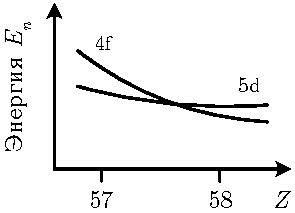
\includegraphics[width=4cm]{figs/rules_for_filling_electronic_shells/4f_and_5d_levels.pdf}
        \end{figure}
    \end{sol}
\end{problem}